\documentclass[noragright,centerchapter,12pt]{uiucecethesis09}
% Use draftthesis for notes and date markings on every page.  Useful when you
%   have multiple copies floating around.
% Use offcenter for the extra .5 inch on the left side. Needed with fullpage and fancy.
% Use mixcasechap for compatibility with hyperref package, which does NOT like all caps default
% Use edeposit for the adviser/committee on the title page.
% Use tocnosub to suppress subsection and lower entries in the TOC.
% PhD candidates use "proquest" for the proquest abstract.

\makeatletter

\usepackage[acronym,toc]{glossaries}
%\newacronym{<++>}{<++>}{<++>}
\newacronym[longplural={metric tons of heavy metal}]{MTHM}{MTHM}{metric ton of heavy metal}
\newacronym[longplural={metric tons of initial heavy metal}]{MTIHM}{MTIHM}{metric ton of initial heavy metal}
\newacronym{ABM}{ABM}{agent-based modeling}
\newacronym{ACDIS}{ACDIS}{Program in Arms Control \& Domestic and International Security}
\newacronym{AHTR}{AHTR}{Advanced High Temperature Reactor}
\newacronym{ANDRA}{ANDRA}{Agence Nationale pour la gestion des D\'echets RAdioactifs, the French National Agency for Radioactive Waste Management}
\newacronym{ANL}{ANL}{Argonne National Laboratory}
\newacronym{API}{API}{application programming interface}
\newacronym{ARCH}{ARCH}{autoregressive conditional heteroskedastic}
\newacronym{ARE}{ARE}{Aircraft Reactor Experiment}
\newacronym{ARFC}{ARFC}{Advanced Reactors and Fuel Cycles}
\newacronym{ARMA}{ARMA}{autoregressive moving average}
\newacronym{ASME}{ASME}{American Society of Mechanical Engineers}
\newacronym{ATWS}{ATWS}{Anticipated Transient Without Scram}
\newacronym{BDBE}{BDBE}{Beyond Design Basis Event}
\newacronym{BIDS}{BIDS}{Berkeley Institute for Data Science}
\newacronym{BOL}{BOL}{Beginning-of-Life}
\newacronym{BSD}{BSD}{Berkeley Software Distribution}
\newacronym{CAFCA}{CAFCA}{ Code for Advanced Fuel Cycles Assessment }
\newacronym{CASL}{CASL}{Consortium for Advanced Simulation of Light Water Reactors}
\newacronym{CDTN}{CDTN}{Centro de Desenvolvimento da Tecnologia Nuclear}
\newacronym{CEA}{CEA}{Commissariat \`a l'\'Energie Atomique et aux \'Energies Alternatives}
\newacronym{CI}{CI}{continuous integration}
\newacronym{CNEC}{CNEC}{Consortium for Nonproliferation Enabling Capabilities}
\newacronym{CNEN}{CNEN}{Comiss\~{a}o Nacional de Energia Nuclear}
\newacronym{CNERG}{CNERG}{Computational Nuclear Engineering Research Group}
\newacronym{COSI}{COSI}{Commelini-Sicard}
\newacronym{COTS}{COTS}{commercial, off-the-shelf}
\newacronym{CSNF}{CSNF}{commercial spent nuclear fuel}
\newacronym{CTAH}{CTAHs}{Coiled Tube Air Heaters}
\newacronym{CUBIT}{CUBIT}{CUBIT Geometry and Mesh Generation Toolkit}
\newacronym{CURIE}{CURIE}{Centralized Used Fuel Resource for Information Exchange}
\newacronym{DAG}{DAG}{directed acyclic graph}
\newacronym{DANESS}{DANESS}{Dynamic Analysis of Nuclear Energy System Strategies}
\newacronym{DBE}{DBE}{Design Basis Event}
\newacronym{DESAE}{DESAE}{Dynamic Analysis of Nuclear Energy Systems Strategies}
\newacronym{DHS}{DHS}{Department of Homeland Security}
\newacronym{DOE}{DOE}{Department of Energy}
\newacronym{DRACS}{DRACS}{Direct Reactor Auxiliary Cooling System}
\newacronym{DRE}{DRE}{dynamic resource exchange}
\newacronym{DSNF}{DSNF}{DOE spent nuclear fuel}
\newacronym{DYMOND}{DYMOND}{Dynamic Model of Nuclear Development }
\newacronym{EBS}{EBS}{Engineered Barrier System}
\newacronym{EDZ}{EDZ}{Excavation Disturbed Zone}
\newacronym{EIA}{EIA}{U.S. Energy Information Administration}
\newacronym{EPA}{EPA}{Environmental Protection Agency}
\newacronym{EP}{EP}{Engineering Physics}
\newacronym{FCO}{FCO}{Fuel Cycle Options}
\newacronym{FCT}{FCT}{Fuel Cycle Technology}
\newacronym{FCWMD}{FCWMD}{Fuel Cycle and Waste Management Division}
\newacronym{FEHM}{FEHM}{Finite Element Heat and Mass Transfer}
\newacronym{FEPs}{FEPs}{Features, Events, and Processes}
\newacronym{FHR}{FHR}{Fluoride-Salt-Cooled High-Temperature Reactor}
\newacronym{FLiBe}{FLiBe}{Fluoride-Lithium-Beryllium}
\newacronym{GCAM}{GCAM}{Global Change Assessment Model}
\newacronym{GDSE}{GDSE}{Generic Disposal System Environment}
\newacronym{GDSM}{GDSM}{Generic Disposal System Model}
\newacronym{GENIUSv1}{GENIUSv1}{Global Evaluation of Nuclear Infrastructure Utilization Scenarios, Version 1}
\newacronym{GENIUSv2}{GENIUSv2}{Global Evaluation of Nuclear Infrastructure Utilization Scenarios, Version 2}
\newacronym{GENIUS}{GENIUS}{Global Evaluation of Nuclear Infrastructure Utilization Scenarios}
\newacronym{GPAM}{GPAM}{Generic Performance Assessment Model}
\newacronym{GRSAC}{GRSAC}{Graphite Reactor Severe Accident Code}
\newacronym{GUI}{GUI}{graphical user interface}
\newacronym{GWd}{GWd}{Gigawatt Days}
\newacronym{HLW}{HLW}{high level waste}
\newacronym{HPC}{HPC}{high-performance computing}
\newacronym{HTC}{HTC}{high-throughput computing}
\newacronym{HTGR}{HTGR}{High Temperature Gas-Cooled Reactor}
\newacronym{IAEA}{IAEA}{International Atomic Energy Agency}
\newacronym{IEMA}{IEMA}{Illinois Emergency Mangament Agency}
\newacronym{INL}{INL}{Idaho National Laboratory}
\newacronym{IPRR1}{IRP-R1}{Instituto de Pesquisas Radioativas Reator 1}
\newacronym{IRP}{IRP}{Integrated Research Project}
\newacronym{ISFSI}{ISFSI}{Independent Spent Fuel Storage Installation}
\newacronym{ISRG}{ISRG}{Independent Student Research Group}
\newacronym{JFNK}{JFNK}{Jacobian-Free Newton Krylov}
\newacronym{KAERI}{KAERI}{Korea Atomic Energy Research Institute}
\newacronym{LANL}{LANL}{Los Alamos National Laboratory}
\newacronym{LBNL}{LBNL}{Lawrence Berkeley National Laboratory}
\newacronym{LCOE}{LCOE}{levelized cost of electricity}
\newacronym{LDRD}{LDRD}{laboratory directed research and development}
\newacronym{LFR}{LFR}{Lead-Cooled Fast Reactor}
\newacronym{LGPL}{LGPL}{Lesser GNU Public License}
\newacronym{LLNL}{LLNL}{Lawrence Livermore National Laboratory}
\newacronym{LMFBR}{LMFBR}{Liquid-Metal-cooled Fast Breeder Reactor}
\newacronym{LOFC}{LOFC}{Loss of Forced Cooling}
\newacronym{LOHS}{LOHS}{Loss of Heat Sink}
\newacronym{LOLA}{LOLA}{Loss of Large Area}
\newacronym{LP}{LP}{linear program}
\newacronym{LWR}{LWR}{Light Water Reactor}
\newacronym{MARKAL}{MARKAL}{MARKet and ALlocation}
\newacronym{MA}{MA}{minor actinide}
\newacronym{MCNP}{MCNP}{Monte Carlo N-Particle code}
\newacronym{MILP}{MILP}{mixed-integer linear program}
\newacronym{MIT}{MIT}{the Massachusetts Institute of Technology}
\newacronym{MOAB}{MOAB}{Mesh-Oriented datABase}
\newacronym{MOOSE}{MOOSE}{Multiphysics Object-Oriented Simulation Environment}
\newacronym{MOX}{MOX}{mixed oxide}
\newacronym{MSBR}{MSBR}{Molten Salt Breeder Reactor}
\newacronym{MSRE}{MSRE}{Molten Salt Reactor Experiment}
\newacronym{MSR}{MSR}{Molten Salt Reactor}
\newacronym{MWd}{MWd}{Megawatt Days}
\newacronym{NAGRA}{NAGRA}{National Cooperative for the Disposal of Radioactive Waste}
\newacronym{NCSA}{NCSA}{National Center for Supercomputing Applications}
\newacronym{NEAMS}{NEAMS}{Nuclear Engineering Advanced Modeling and Simulation}
\newacronym{NEUP}{NEUP}{Nuclear Energy University Programs}
\newacronym{NFCSim}{NFCSim}{Nuclear Fuel Cycle Simulator}
\newacronym{NFC}{NFC}{Nuclear Fuel Cycle}
\newacronym{NGNP}{NGNP}{Next Generation Nuclear Plant}
\newacronym{NMWPC}{NMWPC}{Nuclear MW Per Capita}
\newacronym{NNSA}{NNSA}{National Nuclear Security Administration}
\newacronym{NPRE}{NPRE}{Department of Nuclear, Plasma, and Radiological Engineering}
\newacronym{NQA1}{NQA-1}{Nuclear Quality Assurance - 1}
\newacronym{NRC}{NRC}{Nuclear Regulatory Commission}
\newacronym{NSF}{NSF}{National Science Foundation}
\newacronym{NSSC}{NSSC}{Nuclear Science and Security Consortium}
\newacronym{NUWASTE}{NUWASTE}{Nuclear Waste Assessment System for Technical Evaluation}
\newacronym{NWF}{NWF}{Nuclear Waste Fund}
\newacronym{NWTRB}{NWTRB}{Nuclear Waste Technical Review Board}
\newacronym{OCRWM}{OCRWM}{Office of Civilian Radioactive Waste Management}
\newacronym{ORION}{ORION}{ORION}
\newacronym{ORNL}{ORNL}{Oak Ridge National Laboratory}
\newacronym{PARCS}{PARCS}{Purdue Advanced Reactor Core Simulator}
\newacronym{PBAHTR}{PB-AHTR}{Pebble Bed Advanced High Temperature Reactor}
\newacronym{PBFHR}{PB-FHR}{Pebble-Bed Fluoride-Salt-Cooled High-Temperature Reactor}
\newacronym{PEI}{PEI}{Peak Environmental Impact}
\newacronym{PH}{PRONGHORN}{PRONGHORN}
\newacronym{PI}{PI}{Principal Investigator}
\newacronym{PNNL}{PNNL}{Pacific Northwest National Laboratory}
\newacronym{PRIDE}{PRIDE}{Pyroprocessing Integrated Demonstration}
\newacronym{PRKE}{PRKE}{Point Reactor Kinetics Equations}
\newacronym{PSPG}{PSPG}{Pressure-Stabilizing/Petrov-Galerkin}
\newacronym{PWAR}{PWAR}{Pratt and Whitney Aircraft Reactor}
\newacronym{PWR}{PWR}{Pressurized Water Reactor}
\newacronym{PyNE}{PyNE}{Python toolkit for Nuclear Engineering}
\newacronym{PyRe}{PyRe}{Pyro Reprocessing Module}
\newacronym{PyRK}{PyRK}{Python for Reactor Kinetics}
\newacronym{QA}{QA}{quality assurance}
\newacronym{RDD}{RD\&D}{Research Development and Demonstration}
\newacronym{RD}{R\&D}{Research and Development}
\newacronym{RELAP}{RELAP}{Reactor Excursion and Leak Analysis Program}
\newacronym{RIA}{RIA}{Reactivity Insertion Accident}
\newacronym{RIF}{RIF}{Region-Institution-Facility}
\newacronym{SAM}{SAM}{Simulation and Modeling}
\newacronym{SCF}{SCF}{Software Carpentry Foundation}
\newacronym{SFR}{SFR}{Sodium-Cooled Fast Reactor}
\newacronym{SINDAG}{SINDA{\textbackslash}G}{Systems Improved Numerical Differencing Analyzer $\backslash$ Gaski}
\newacronym{SKB}{SKB}{Svensk K\"{a}rnbr\"{a}nslehantering AB}
\newacronym{SNF}{SNF}{spent nuclear fuel}
\newacronym{SNL}{SNL}{Sandia National Laboratory}
\newacronym{SNM}{SNM}{Special Nuclear Material}
\newacronym{STC}{STC}{specific temperature change}
\newacronym{SUPG}{SUPG}{Streamline-Upwind/Petrov-Galerkin}
\newacronym{SWF}{SWF}{Separations and Waste Forms}
\newacronym{SWU}{SWU}{Separative Work Unit}
\newacronym{SandO}{S\&O}{Signatures and Observables}
\newacronym{THW}{THW}{The Hacker Within}
\newacronym{TRIGA}{TRIGA}{Training Research Isotope General Atomic}
\newacronym{TRISO}{TRISO}{Tristructural Isotropic}
\newacronym{TRU}{TRU}{transuranic} 
\newacronym{TSM}{TSM}{Total System Model}
\newacronym{TSPA}{TSPA}{Total System Performance Assessment for the Yucca Mountain License Application}
\newacronym{UFD}{UFD}{Used Fuel Disposition}
\newacronym{UML}{UML}{Unified Modeling Language}
\newacronym{UOX}{UOX}{uranium oxide}
\newacronym{UQ}{UQ}{uncertainty quantification}
\newacronym{US}{US}{United States}
\newacronym{UW}{UW}{University of Wisconsin}
\newacronym{VISION}{VISION}{the Verifiable Fuel Cycle Simulation Model}
\newacronym{VV}{V\&V}{verification and validation}
\newacronym{WIPP}{WIPP}{Waste Isolation Pilot Plant}
\newacronym{YMG}{YMG}{Young Members Group}
\newacronym{YMR}{YMR}{Yucca Mountain Repository Site}


\usepackage{xspace}

\newcommand{\Cycamore}{\textsc{Cycamore}\xspace}
\newcommand{\Cyclus}{\textsc{Cyclus}\xspace}

\usepackage{url}
\usepackage{setspace}
%\usepackage{epsfig}  % for figures
\usepackage{graphicx}  % another package that works for figures
\usepackage{multirow}
\usepackage{placeins}
\usepackage{caption}  % allows center figures caption
\usepackage{booktabs} % nice rules (thick lines) for tables
\usepackage{array}
\usepackage{tabularx}
\graphicspath{{figures/}}
%\usepackage{subfigure}  % for subfigures
\usepackage{amsmath}  % for math spacing
%\usepackage{amssymb}  % for math spacing
%\usepackage{url}  % Hyphenation of URLs.
\usepackage{lscape}  % Useful for wide tables or figures.
\usepackage[justification=raggedright]{caption}	% makes captions ragged right - thanks to Bryce Lobdell
\usepackage{color,soul}
\makeglossary

% Uncomment the appropriate one of the following four lines:
\msthesis
%\phdthesis
%\otherdoctorate[abbrev]{Title of Degree}
%\othermasters[abbrev]{Title of Degree}

\title{Online Diversion Detection in Cyclus}
\author{Greg T. Westphal}
\department{Nuclear, Plasma, and Radiological Engineering}
\degreeyear{2019}

% Advisor name is required for
% - doctoral students for the ProQuest abstract
% - master's students who do not have a master's committee
%\advisor{Professor Kathryn D. Huff}

% Uncomment the \committee command for
% - all doctoral students
% - master's students who have a master's committee
\committee{Assistant Professor Kathryn Huff, Chair\\
           Unknown Professor} % etc.

\begin{document}
%\newacronym{<++>}{<++>}{<++>}
\newacronym[longplural={metric tons of heavy metal}]{MTHM}{MTHM}{metric ton of heavy metal}
\newacronym[longplural={metric tons of initial heavy metal}]{MTIHM}{MTIHM}{metric ton of initial heavy metal}
\newacronym{ABM}{ABM}{agent-based modeling}
\newacronym{ACDIS}{ACDIS}{Program in Arms Control \& Domestic and International Security}
\newacronym{AHTR}{AHTR}{Advanced High Temperature Reactor}
\newacronym{ANDRA}{ANDRA}{Agence Nationale pour la gestion des D\'echets RAdioactifs, the French National Agency for Radioactive Waste Management}
\newacronym{ANL}{ANL}{Argonne National Laboratory}
\newacronym{API}{API}{application programming interface}
\newacronym{ARCH}{ARCH}{autoregressive conditional heteroskedastic}
\newacronym{ARE}{ARE}{Aircraft Reactor Experiment}
\newacronym{ARFC}{ARFC}{Advanced Reactors and Fuel Cycles}
\newacronym{ARMA}{ARMA}{autoregressive moving average}
\newacronym{ASME}{ASME}{American Society of Mechanical Engineers}
\newacronym{ATWS}{ATWS}{Anticipated Transient Without Scram}
\newacronym{BDBE}{BDBE}{Beyond Design Basis Event}
\newacronym{BIDS}{BIDS}{Berkeley Institute for Data Science}
\newacronym{BOL}{BOL}{Beginning-of-Life}
\newacronym{BSD}{BSD}{Berkeley Software Distribution}
\newacronym{CAFCA}{CAFCA}{ Code for Advanced Fuel Cycles Assessment }
\newacronym{CASL}{CASL}{Consortium for Advanced Simulation of Light Water Reactors}
\newacronym{CDTN}{CDTN}{Centro de Desenvolvimento da Tecnologia Nuclear}
\newacronym{CEA}{CEA}{Commissariat \`a l'\'Energie Atomique et aux \'Energies Alternatives}
\newacronym{CI}{CI}{continuous integration}
\newacronym{CNEC}{CNEC}{Consortium for Nonproliferation Enabling Capabilities}
\newacronym{CNEN}{CNEN}{Comiss\~{a}o Nacional de Energia Nuclear}
\newacronym{CNERG}{CNERG}{Computational Nuclear Engineering Research Group}
\newacronym{COSI}{COSI}{Commelini-Sicard}
\newacronym{COTS}{COTS}{commercial, off-the-shelf}
\newacronym{CSNF}{CSNF}{commercial spent nuclear fuel}
\newacronym{CTAH}{CTAHs}{Coiled Tube Air Heaters}
\newacronym{CUBIT}{CUBIT}{CUBIT Geometry and Mesh Generation Toolkit}
\newacronym{CURIE}{CURIE}{Centralized Used Fuel Resource for Information Exchange}
\newacronym{DAG}{DAG}{directed acyclic graph}
\newacronym{DANESS}{DANESS}{Dynamic Analysis of Nuclear Energy System Strategies}
\newacronym{DBE}{DBE}{Design Basis Event}
\newacronym{DESAE}{DESAE}{Dynamic Analysis of Nuclear Energy Systems Strategies}
\newacronym{DHS}{DHS}{Department of Homeland Security}
\newacronym{DOE}{DOE}{Department of Energy}
\newacronym{DRACS}{DRACS}{Direct Reactor Auxiliary Cooling System}
\newacronym{DRE}{DRE}{dynamic resource exchange}
\newacronym{DSNF}{DSNF}{DOE spent nuclear fuel}
\newacronym{DYMOND}{DYMOND}{Dynamic Model of Nuclear Development }
\newacronym{EBS}{EBS}{Engineered Barrier System}
\newacronym{EDZ}{EDZ}{Excavation Disturbed Zone}
\newacronym{EIA}{EIA}{U.S. Energy Information Administration}
\newacronym{EPA}{EPA}{Environmental Protection Agency}
\newacronym{EP}{EP}{Engineering Physics}
\newacronym{FCO}{FCO}{Fuel Cycle Options}
\newacronym{FCT}{FCT}{Fuel Cycle Technology}
\newacronym{FCWMD}{FCWMD}{Fuel Cycle and Waste Management Division}
\newacronym{FEHM}{FEHM}{Finite Element Heat and Mass Transfer}
\newacronym{FEPs}{FEPs}{Features, Events, and Processes}
\newacronym{FHR}{FHR}{Fluoride-Salt-Cooled High-Temperature Reactor}
\newacronym{FLiBe}{FLiBe}{Fluoride-Lithium-Beryllium}
\newacronym{GCAM}{GCAM}{Global Change Assessment Model}
\newacronym{GDSE}{GDSE}{Generic Disposal System Environment}
\newacronym{GDSM}{GDSM}{Generic Disposal System Model}
\newacronym{GENIUSv1}{GENIUSv1}{Global Evaluation of Nuclear Infrastructure Utilization Scenarios, Version 1}
\newacronym{GENIUSv2}{GENIUSv2}{Global Evaluation of Nuclear Infrastructure Utilization Scenarios, Version 2}
\newacronym{GENIUS}{GENIUS}{Global Evaluation of Nuclear Infrastructure Utilization Scenarios}
\newacronym{GPAM}{GPAM}{Generic Performance Assessment Model}
\newacronym{GRSAC}{GRSAC}{Graphite Reactor Severe Accident Code}
\newacronym{GUI}{GUI}{graphical user interface}
\newacronym{GWd}{GWd}{Gigawatt Days}
\newacronym{HLW}{HLW}{high level waste}
\newacronym{HPC}{HPC}{high-performance computing}
\newacronym{HTC}{HTC}{high-throughput computing}
\newacronym{HTGR}{HTGR}{High Temperature Gas-Cooled Reactor}
\newacronym{IAEA}{IAEA}{International Atomic Energy Agency}
\newacronym{IEMA}{IEMA}{Illinois Emergency Mangament Agency}
\newacronym{INL}{INL}{Idaho National Laboratory}
\newacronym{IPRR1}{IRP-R1}{Instituto de Pesquisas Radioativas Reator 1}
\newacronym{IRP}{IRP}{Integrated Research Project}
\newacronym{ISFSI}{ISFSI}{Independent Spent Fuel Storage Installation}
\newacronym{ISRG}{ISRG}{Independent Student Research Group}
\newacronym{JFNK}{JFNK}{Jacobian-Free Newton Krylov}
\newacronym{KAERI}{KAERI}{Korea Atomic Energy Research Institute}
\newacronym{LANL}{LANL}{Los Alamos National Laboratory}
\newacronym{LBNL}{LBNL}{Lawrence Berkeley National Laboratory}
\newacronym{LCOE}{LCOE}{levelized cost of electricity}
\newacronym{LDRD}{LDRD}{laboratory directed research and development}
\newacronym{LFR}{LFR}{Lead-Cooled Fast Reactor}
\newacronym{LGPL}{LGPL}{Lesser GNU Public License}
\newacronym{LLNL}{LLNL}{Lawrence Livermore National Laboratory}
\newacronym{LMFBR}{LMFBR}{Liquid-Metal-cooled Fast Breeder Reactor}
\newacronym{LOFC}{LOFC}{Loss of Forced Cooling}
\newacronym{LOHS}{LOHS}{Loss of Heat Sink}
\newacronym{LOLA}{LOLA}{Loss of Large Area}
\newacronym{LP}{LP}{linear program}
\newacronym{LWR}{LWR}{Light Water Reactor}
\newacronym{MARKAL}{MARKAL}{MARKet and ALlocation}
\newacronym{MA}{MA}{minor actinide}
\newacronym{MCNP}{MCNP}{Monte Carlo N-Particle code}
\newacronym{MILP}{MILP}{mixed-integer linear program}
\newacronym{MIT}{MIT}{the Massachusetts Institute of Technology}
\newacronym{MOAB}{MOAB}{Mesh-Oriented datABase}
\newacronym{MOOSE}{MOOSE}{Multiphysics Object-Oriented Simulation Environment}
\newacronym{MOX}{MOX}{mixed oxide}
\newacronym{MSBR}{MSBR}{Molten Salt Breeder Reactor}
\newacronym{MSRE}{MSRE}{Molten Salt Reactor Experiment}
\newacronym{MSR}{MSR}{Molten Salt Reactor}
\newacronym{MWd}{MWd}{Megawatt Days}
\newacronym{NAGRA}{NAGRA}{National Cooperative for the Disposal of Radioactive Waste}
\newacronym{NCSA}{NCSA}{National Center for Supercomputing Applications}
\newacronym{NEAMS}{NEAMS}{Nuclear Engineering Advanced Modeling and Simulation}
\newacronym{NEUP}{NEUP}{Nuclear Energy University Programs}
\newacronym{NFCSim}{NFCSim}{Nuclear Fuel Cycle Simulator}
\newacronym{NFC}{NFC}{Nuclear Fuel Cycle}
\newacronym{NGNP}{NGNP}{Next Generation Nuclear Plant}
\newacronym{NMWPC}{NMWPC}{Nuclear MW Per Capita}
\newacronym{NNSA}{NNSA}{National Nuclear Security Administration}
\newacronym{NPRE}{NPRE}{Department of Nuclear, Plasma, and Radiological Engineering}
\newacronym{NQA1}{NQA-1}{Nuclear Quality Assurance - 1}
\newacronym{NRC}{NRC}{Nuclear Regulatory Commission}
\newacronym{NSF}{NSF}{National Science Foundation}
\newacronym{NSSC}{NSSC}{Nuclear Science and Security Consortium}
\newacronym{NUWASTE}{NUWASTE}{Nuclear Waste Assessment System for Technical Evaluation}
\newacronym{NWF}{NWF}{Nuclear Waste Fund}
\newacronym{NWTRB}{NWTRB}{Nuclear Waste Technical Review Board}
\newacronym{OCRWM}{OCRWM}{Office of Civilian Radioactive Waste Management}
\newacronym{ORION}{ORION}{ORION}
\newacronym{ORNL}{ORNL}{Oak Ridge National Laboratory}
\newacronym{PARCS}{PARCS}{Purdue Advanced Reactor Core Simulator}
\newacronym{PBAHTR}{PB-AHTR}{Pebble Bed Advanced High Temperature Reactor}
\newacronym{PBFHR}{PB-FHR}{Pebble-Bed Fluoride-Salt-Cooled High-Temperature Reactor}
\newacronym{PEI}{PEI}{Peak Environmental Impact}
\newacronym{PH}{PRONGHORN}{PRONGHORN}
\newacronym{PI}{PI}{Principal Investigator}
\newacronym{PNNL}{PNNL}{Pacific Northwest National Laboratory}
\newacronym{PRIDE}{PRIDE}{Pyroprocessing Integrated Demonstration}
\newacronym{PRKE}{PRKE}{Point Reactor Kinetics Equations}
\newacronym{PSPG}{PSPG}{Pressure-Stabilizing/Petrov-Galerkin}
\newacronym{PWAR}{PWAR}{Pratt and Whitney Aircraft Reactor}
\newacronym{PWR}{PWR}{Pressurized Water Reactor}
\newacronym{PyNE}{PyNE}{Python toolkit for Nuclear Engineering}
\newacronym{PyRe}{PyRe}{Pyro Reprocessing Module}
\newacronym{PyRK}{PyRK}{Python for Reactor Kinetics}
\newacronym{QA}{QA}{quality assurance}
\newacronym{RDD}{RD\&D}{Research Development and Demonstration}
\newacronym{RD}{R\&D}{Research and Development}
\newacronym{RELAP}{RELAP}{Reactor Excursion and Leak Analysis Program}
\newacronym{RIA}{RIA}{Reactivity Insertion Accident}
\newacronym{RIF}{RIF}{Region-Institution-Facility}
\newacronym{SAM}{SAM}{Simulation and Modeling}
\newacronym{SCF}{SCF}{Software Carpentry Foundation}
\newacronym{SFR}{SFR}{Sodium-Cooled Fast Reactor}
\newacronym{SINDAG}{SINDA{\textbackslash}G}{Systems Improved Numerical Differencing Analyzer $\backslash$ Gaski}
\newacronym{SKB}{SKB}{Svensk K\"{a}rnbr\"{a}nslehantering AB}
\newacronym{SNF}{SNF}{spent nuclear fuel}
\newacronym{SNL}{SNL}{Sandia National Laboratory}
\newacronym{SNM}{SNM}{Special Nuclear Material}
\newacronym{STC}{STC}{specific temperature change}
\newacronym{SUPG}{SUPG}{Streamline-Upwind/Petrov-Galerkin}
\newacronym{SWF}{SWF}{Separations and Waste Forms}
\newacronym{SWU}{SWU}{Separative Work Unit}
\newacronym{SandO}{S\&O}{Signatures and Observables}
\newacronym{THW}{THW}{The Hacker Within}
\newacronym{TRIGA}{TRIGA}{Training Research Isotope General Atomic}
\newacronym{TRISO}{TRISO}{Tristructural Isotropic}
\newacronym{TRU}{TRU}{transuranic} 
\newacronym{TSM}{TSM}{Total System Model}
\newacronym{TSPA}{TSPA}{Total System Performance Assessment for the Yucca Mountain License Application}
\newacronym{UFD}{UFD}{Used Fuel Disposition}
\newacronym{UML}{UML}{Unified Modeling Language}
\newacronym{UOX}{UOX}{uranium oxide}
\newacronym{UQ}{UQ}{uncertainty quantification}
\newacronym{US}{US}{United States}
\newacronym{UW}{UW}{University of Wisconsin}
\newacronym{VISION}{VISION}{the Verifiable Fuel Cycle Simulation Model}
\newacronym{VV}{V\&V}{verification and validation}
\newacronym{WIPP}{WIPP}{Waste Isolation Pilot Plant}
\newacronym{YMG}{YMG}{Young Members Group}
\newacronym{YMR}{YMR}{Yucca Mountain Repository Site}

%%%%%%%%%%%%%%%%%%%%%%%%%%%%%%%%%%%%%%%%%%%%%%%%%%%%%%%%%%%%%%%%%%%%%%%%%%%%%%%
% TITLE
%
\maketitle

%\raggedright
\parindent 1em%

\frontmatter

%%%%%%%%%%%%%%%%%%%%%%%%%%%%%%%%%%%%%%%%%%%%%%%%%%%%%%%%%%%%%%%%%%%%%%%%%%%%%%%
% ABSTRACT
%
\begin{abstract}
% Put the abstract in a file called "abs.tex" and it'll be inputted here.
\vspace{-0.4in}

As a result of the once-through fuel cycle implemented in the US, used nuclear fuel (UNF) steadily increases. One proposed solution is the transition to a closed nuclear fuel cycle, in which reprocessing reduces build up of UNF. Pyroprocessing is an attractive method for this transition for its capabilities separating both light water reactor (LWR) and metallic fuels, and inherent proliferation resistance. However, unlike aqueous reprocessing plants, industrial pyroprocessing plants do not yet exist. Similar
to safety-by-design in next-generation reactors, reprocessing facilities could be designed with safeguards in mind via safeguards-by-design. Without operational experience, these safeguards-by-design need to be derived through modeling and simulation. 

This thesis develops a medium fidelity generic model, Pyre, capable of simulating a variety of pyroprocessing facility configurations. Pyre also simulates diversion via a diverter class capable of tracking signatures and observables. Rather than only tracking exact material production, we use signatures and observables such as operating temperature, pressure, and current to mimic the capabilities of International Atomic Energy Agency (IAEA) inspections and aid identification of nefarious fuel cycles, or shadow fuel cycles.

These capabilities are verified in a transition scenario of the current US fuel cycle to a sodium fast reactor (SFR) based closed fuel cycle. Key operating parameters are determined through
sensitivity analysis of this scenario, monitoring isotopic changes in material unaccounted for. This work concludes that facility parameters which increase interaction between the salt and waste have more impact on material unaccounted for (MUF). This work also expands the state of the art by exploring the use of sub-facility modeling to increase fuel cycle fidelity.
\end{abstract}

%%%%%%%%%%%%%%%%%%%%%%%%%%%%%%%%%%%%%%%%%%%%%%%%%%%%%%%%%%%%%%%%%%%%%%%%%%%%%%%
% DEDICATION
%
\begin{dedication}
dedication
\end{dedication}

%%%%%%%%%%%%%%%%%%%%%%%%%%%%%%%%%%%%%%%%%%%%%%%%%%%%%%%%%%%%%%%%%%%%%%%%%%%%%%%
% ACKNOWLEDGMENTS
%
% Put acknowledgments in a file called "ack.tex" and it'll be inputted here.
\begin{acknowledgments}
First and foremost I would like to thank my advisor Kathryn Huff for her patient guidance
and introduction to software development, as well as her support troubleshooting along the
way. For their help starting out with \Cyclus, multiple debugging efforts, and much more thank you
to Gwendolyn Chee and Teddy Bae. Also my classmates Roberto Fairhurst, Anshuman Chuabe, Sun Myung Park, and Mark Kamuda whose support was a great help. Finally, thank you to my parents and brothers
for their never-ending support and feedback. This material is based upon work supported by the Department of Energy National
Nuclear Security Administration under Award Number(s) DE-NA0002576 through
the Consortium for Nonproliferation Enabling Capabilities.
\end{acknowledgments}																																				
%%%%%%%%%%%%%%%%%%%%%%%%%%%%%%%%%%%%%%%%%%%%%%%%%%%%%%%%%%%%%%%%%%%%%%%%%%%%%%%
% TABLE OF CONTENTS
%
\tableofcontents

%%%%%%%%%%%%%%%%%%%%%%%%%%%%%%%%%%%%%%%%%%%%%%%%%%%%%%%%%%%%%%%%%%%%%%%%%%%%%%%
% LIST OF TABLES
%
% The List of Tables is not strictly necessary. Omitting the List of Tables will
% simplify the thesis check and reduce the number of corrections.
%\listoftables

%%%%%%%%%%%%%%%%%%%%%%%%%%%%%%%%%%%%%%%%%%%%%%%%%%%%%%%%%%%%%%%%%%%%%%%%%%%%%%%
% LIST OF FIGURES
%
% The List of Figures is not strictly necessary. Omitting the List of Figures will
% simplify the thesis check and reduce the number of corrections.
%\listoffigures

%%%%%%%%%%%%%%%%%%%%%%%%%%%%%%%%%%%%%%%%%%%%%%%%%%%%%%%%%%%%%%%%%%%%%%%%%%%%%%%
% LIST OF ABBREVIATIONS
%
% The List of Abbreviations is not strictly necessary.
%\chapter{LIST OF ABBREVIATIONS}

%\printacronyms
%\begin{symbollist*}
%\item[MSBR] Molten Salt Breeder Reactor
%\item[MSR] Molten Salt Reactor
%\item[ORNL] Oak Ridge National Laboratory
%\end{symbollist*}


%%%%%%%%%%%%%%%%%%%%%%%%%%%%%%%%%%%%%%%%%%%%%%%%%%%%%%%%%%%%%%%%%%%%%%%%%%%%%%%
% LIST OF SYMBOLS
%
%\begin{symbollist}[0.7in]
%\item[$\tau$] Time taken to drink one cup of coffee.
%\end{symbollist}

\mainmatter

%%%%%%%%%%%%%%%%%%%%%%%%%%%%%%%%%%%%%%%%%%%%%%%%%%%%%%%%%%%%%%%%%%%%%%%%%%%%%%%
% INSERT REAL CONTENT HERE
%
\chapter[Introduction]{Introduction}
The diversion of significant quantities of \gls{SNM} from the nuclear fuel cycle is major non-proliferation 
concern \cite{noauthor_serving_2017}. These diversions must be detected in a timely manner using signatures and observables in 
order to properly safegaurd the fuel cycle. Timely detection is critical in non-proliferation to discover these shadow fuel cycles
before diverted material is further processed. Pyroprocessing is a used nuclear fuel separations technology for advanced reactors. 
Signatures and observables are used to detect diversion of nuclear material.
The goal of this research is to identify potential signs of material diversion in a pyroprocessing facility and implement models 
of these processes into a detailed pyroprocessing facility archetype to the modular, agent-based, fuel cycle simulator, \Cyclus \cite{huff_fundamental_2016}. This facility archetype will equip users of the \Cyclus fuel cycle simulator to investigate 
detection timeliness enabled by measuring signatures and observables in various fuel cycle scenarios.
\section{Motivation}
\subsection{Safeguards}
Currently there are no commercially operated pyroprocessing plants, however various research designs exist in national labs.
Notably Argonne National Lab, Idaho National Lab and, in South Korea, KAERI \cite{michael_f._simpson_developments_2012, lee_advanced, frigo_conceptual_2003}. 
Therefore, prior to construction of any design we 
want to implement safeguards by design. Similar to security by design in next generation reactors, the goal is to include key measurement 
points and access points to the design of the facility. Rather than learn from mistakes, in the future we aim to incorporate safety 
into the design.

\subsection{Pyroprocessing}
For other fuel cycle facilities, we have plenty of operating experience to inform on safeguard construction. For example, with aqueous reprocessing
the IAEA provides detailed flowsheets of example facilities \cite{international_atomic_energy_agency_implications_2004}. To combat this, multiple modeling
tools have been developed for electrochemical processes such as SSPM and AMPYRE \cite{}. These tools take a high fidelity approach to model the
chemistry taking place within each chamber. In order to run these tools, the user must have intimate knowlege of the specific facility the flowsheets have
been designed for. There is a gap, however, in the medium fidelity models that can inform on broader fuel cycle applications. A generic facility
capable of modeling changes in operational settings and various layouts has not yet been implemented to a fuel cycle simulator \cite{borrelli_approaches_2017}.


\subsection{Future Fuel Cycles}

\paragraph{As public concern for nuclear power focuses on waste, we need to look closer at closed fuel cycles.}

\paragraph{Pyroprocessing can transition between current fuel cycle scenarios with light water reactors and SFRs and other metallic fuel.}


\section{Background}
\subsection{Pyroprocessing}
Pyroprocessing is an electrochemical separation method used primarily for metallic fast reactor fuel.
This reprocessing technique uses molten salt, which differs depending on the facility, to provide a medium for current to travel across.
Molten salt such as LiCl-KCl has a broader stability range comparative to water, allowing high potentials to be used for separation.
Traditionally, separation would be conducted in a nitric acid which uses water as its medium.
Water, however, has a significantly lower stability compared to molten salt.
This becomes a problem when considering higher elements such as lanthanides and actinides.
Controlling the oxidation states of these elements often requires potentials outside the stability of water.
Hence, Pyroprocessing was born to improve nonproliferation and reprocessing capabilities.
\\ \\
In addition to the additional redox control of higher elements, we also co-extract materials of interest such that they cannot easily be refined for weapons.
This is done through the electrorefining and electrowinning stages by separating a pure Uranium stream as well as a Uranium/Transuranic mix stream. 
The U/TRU can then be readily used for fuel fabrication while maintaining proliferation resistance.

\subsubsection{Electrochemical Separations}
Electrochemical separation is the driving force behind pyroprocessing. Electrochemistry relies on the use of Gibbs free energy to determine the required amount of energy to drive a reaction forward.

\begin{figure}[h]
	\centering
	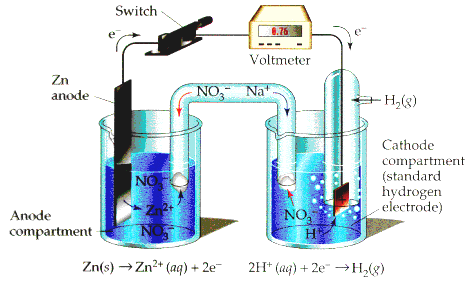
\includegraphics[width=0.8\linewidth]{images/electrochem}
	\caption{Basic example of movement of ion within galvanic cell \cite{angel}.}
	\label{fig:electrochem}
\end{figure}

Figure \ref{fig:electrochem} demonstrates an electrochemical process that generates electricity as a basic example.
The processes described here follow the same principles, however, require energy to run.
In both cases, ions are exchanged between the anode and cathode in an attempt to balance the potential difference.
In the case of pyroprocessing, the potential difference is artificially applied.
A number of different anodes and cathodes are used to force the desired ions to deliver charge from one end of the cell to the other.
These ions that collect on the surface of the cathode can then be removed from the liquid and separated from the rest of the solution.
By controlling the voltage of the solution as well as the composition of the anode, cathode, and electrolyte we can ensure the removal of unwanted elements/isotopes.


\subsubsection{Voloxidation}
Voloxidation is used following the chopping and decladding of the spent fuel. The process is very similar to annealing in regards to materials. The Uranium dioxide is heated to temperatures around 700-1000$^\circ C$ which allows gases and some fission products to escape the fuel pellet. UO$_2$ is converted to U$_3$O$_8$ in this process as well\cite{organisation}. Voloxidation, in most cases, takes place in air which provides plenty of oxygen for oxidization of solid UO$_2$ \cite{jubin_spent_2009}:

\[ 3UO_2 + O_2 \rightarrow U_3O_8 \]

The above reaction is possible because of the expansion of uranium at elevated temperatures. A positive feedback is also established as the Uranium dioxide converts to yellowcake powder, the fuel element expands exposing more Uranium dioxide to oxygen. The rate of this reaction/conversion is dependent on the temperature and gas used. Higher temperatures will yield a faster reaction rate, however, even ~500 $^\circ C$ is sufficient for 99\% reduction in 4 hours.

An added benefit of running a pyroprocessing voloxidation sub-process at the temperatures previously mentioned, 700-1000$^\circ C$, is the removal of some fission products. The PRIDE facility at KAERI takes it a step further and voloxidates at 1250$^\circ C$ to remove troublesome fission products at the beginning of the cycle\cite{organisation}:

\[ 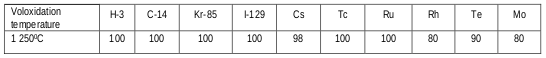
\includegraphics[width=\linewidth]{images/volox_table.png} \]

As shown in the table above, a majority of high activity isotopes are removed from the system at the beginning of pyroprocessing. This protects equipment and workers down the line. These gases are sent to the off-gas treatment facility that makes use of various scrubbing techniques such as liquid scrubbing, cyrogenic distillation (for the krypton), caustic scrubbing, etc \cite{jubin_spent_2009}.

\subsubsection{Electroreduction}
Following off-gassing and conversion to yellowcake, the non-metallic fuel must be converted and reduced to molten salt mixture. Most cases this is done with a LiCl-KCl salt eutectic combined with Li$_2$O catalyst. The electrolytic reduction phase consists of three main parts: UO$_2$ recovery, reduction, and RE removal.

\begin{figure}[h]
	\centering
	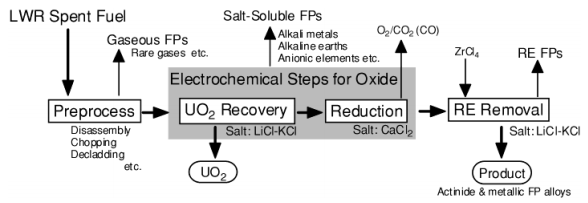
\includegraphics[width=\linewidth]{images/reduction_flow}
	\caption{Electroreduction flow sheet \cite{ohta}.}
\end{figure}

First step in electrolytic reduction is the recovery of UO$_2$ before reducing the remaining material.
The following equations dictate the transfer of Uranium from the anode to the cathode.

\[ UO_2 \rightarrow UO_2^{2+}(LiCl-KCl) + 2e^{2-} \hspace{6mm} anode \]
\[ UO^{2+}(LiCl-KCl) + 2e^{2-} \rightarrow UO_2 \hspace{6mm} cathode \]

As in other separations technologies, noble metals can often follow the uranium through the rest of the process.
The lurking noble metal fission products cause an increase in radioactivity of the UO$_2$ stream. 
Therefore, the weight percent dissolution of Uranium is critical in reducing the amount of waste that follows to the product stream.
Lithium Oxide can also be used as a catalyst to draw Uranium to the cathode while leaving the noble metal fission products in the salt.
This is done with 1-3wt\% Li$_2$O in the following equations \cite{hur_electrochemical_nodate}:

\[ Li_2O \rightarrow 2Li^+ + O^{2-} \]
\[ UO_{x/2} + xLi \rightarrow U + xLi_2O \]

These equations make a continuously driven loop dragging Uranium (either UO$_2$ or U$_3$O$_8$) from the anode to the cathode. 
Disproportionated Lithium ions from the first equation break apart the Uranium and Oxide, with help from the electric potential.
The U will collect on the cathode while the Li$_2$O is recycled and drives the first equation to the right again. 
Reduction then occurs on the cathode where the U, TRU, rare earths and noble metals have collected.
This is achieved by evolving oxygen gas along the anode using the following reactions\cite{hur_electrochemical_nodate,organisation}:

\[ Li^+ \rightarrow Li + e^- \hspace{10mm} Cathode \]
\[ M_xO_y + 2yLi \rightarrow xM + yLi_2O \hspace{10mm} Cathode \]
\[ O^{2-} \rightarrow 0.5O_2 + 2e^- \hspace{10mm} Anode \]

Electrochemical reduction results in an alloy of reduced U/TRU/RE/NM, however, we want to minimize the amount of RE and NM in the product.
We've touched already on how to reduce the quantity of NM and for the final step the RE must be removed.
The RE FPs can be removed from the alloy by substituting another chloride into the LiCl-KCl eutectic.
In the case of Ohta et al. ZrCl$_4$ was considered \cite{ohta}:

\[ 3ZrCl_4(LiCl-KCl + RE \rightarrow 3Zr + 4RECl_3(LiCl-KCl) \]

This process is shown to have a decontamination factor of 10 in regards to separating REs from actinides \cite{sakamura}. Additionally, by using Zirconium as the metal substitute, it is compatible with fuel fabrication later \cite{ohta}.
\subsubsection{Electrorefining}
Electrorefining is the primary process in pyroprocessing, and is the feed point for fast reactor fuel, since it does not require reduction or chopping.
Being the most important process, it is also the most complex with a multitude of input parameters and outputs. 
The goal of the refining process is to separate the Uranium and TRU from the alloy ingot formed in the reduction phase.
Two streams will be formed for the fabrication of fuel. One stream that is a mix of U/TRU at the desired ratio, and the other a pure stream of Uranium.
The refining step's efficiency relies on temperature and current primarily, however, advanced methods are being developed.
KAERI for example has conducted work on adding a central stirrer, vacuum pressure, and rotating the anode \cite{lee_advanced}.
The rotation aims to mix the Uranium in the salt such that none gets stuck on the bottom or edges of the vessel. 
Stirring too vigorously, however, can lead to the removal of uranium dendrites from the cathode thereby decreasing efficiency.\\

The governing reactions that allow this process to work are based on the stability constants and oxidization potential of the remaining fission products.
The voltage used is such that Uranium is unstable in the chloride form, 0.5~1V \cite{organisation}, while transuranics have a higher stability. 
This leads to TRU remaining in chloride form, along with some Uranium, and pure Uranium accumulating on the cathode.
The chloride reaction follows the below equation, and will run to the right as long as there is Uranium within the salt \cite{organisation}.

\[ UCl_3+TRU(RE) \rightarrow U + TRU(RE)Cl_3 \]
\[ UCl_3 + 3Na \rightarrow 3NaCl + U \]
\[ UCl_3 + 3Cs \rightarrow 3CsCl + U \]
\[ UCl_3 + Pu \rightarrow PuCl_3 + U \hspace{10mm} \delta G = -22.44kcal \]
\[ 4UCl_3 + 3Zr \rightarrow 3ZrCl_4 + 5U \hspace{10mm} \delta G = 31.123kcal \]

As shown by the reactions above, the TRU have a favorable gibbs free energy value for spontaneous reaction while the transition metals do not \cite{supy}.
This leads to the transition metals remaining in anode basket while the TRU are drawn into the liquid cadmium cathode \cite{lee_korean_2011}.


\subsubsection{Electrowinning}
The Electrorefiner accumulates TRUs and rare earth fission products within the salt.
These isotopes build up and require separation and disposal, therefore the salt from the refiner is sent to the electrowinner.
This stage further purifies the salt by targeting the electric potential of TRUs, RE and Uranium again \cite{lee_korean_2011,organisation}.
Placed in liquid cadmium once again, the three groups have overlapping electric potentials.
Therefore, the three groups will all deposit in the cadmium \cite{lee_korean_2011}. 
While the refiner's role is to generate a stream of pure Uranium, the electrowinner performs co-extraction of Uranium and TRUs.
This inherit proliferation resistance is a main draw of the pyroprocessing technique.
Rare earths are still present on the cadmium therefore further separations must be conducted.
These elements are removed through the addition of CdCl$_2$ which oxidizes the rare earths while the uranium and TRUs are unaffected.
These oxidized elements fall back into the salt, leaving the purified U/TRU stream on the electrowinner.


Although the facility is great in terms of safeguards, pyroprocessing has its share of drawbacks as well.
Currently, pyroprocessing can only be performed as a batch process, which signficantly limits throughput compared to a continuous facility. 
Additionally, the safety and economical concerns of running a molten salt plant are much greater than a nitric acid one.
Despite these downsides, pyroprocessing is an efficient use of electrochemical separation and leader in proliferation resistant separations.

There are multiple different designs for a pyroprocessing facility, the most prominent being from ANL, INL, and KAERI. In order to encompass them all, we must take a generic approach. This is accomplished by including the following sub-processes: Voloxidation, Electroreduction, Electrorefining, and Electrowinning. While Electrorefining is the process of primary concern, each of the processes has an important in role in various processing plants. 

\section{Goals}

The goals of this work are to appropriately model a generic pyroprocessing facility with medium fidelity capable of diversion. With this model
in \Cyclus we wish to explore the capability of modeling sub-facilities and diversion. In addition, we will use this higher fidelity model to verify transition
scenarios such as EG01-EG24 within \Cyclus \cite{wigeland_nuclear_2014}. Finally we wish to evaluate optimum detector placement and measurement points for
various facility layouts through sensitivity analysis. 	% for INTRODUCTION in "intro.tex"
%\chapter[Methods]{Methods}
\section{Cyclus}

\Cyclus is a modular, agent-based nuclear fuel cycle simulator that models the flow of material through user-defined nuclear fuel cycle scenarios. \Cycamore, the CYClus 
Additional MOdules REpository, provides common facility archetypes (separations, enrichment, reactor, etc.) \cite{carlsen_cycamore_2014}. 
The \Cyclus framework provides benefits compared to other fuel cycle simulators, some being the open source nature, modular capabilities, and use of agents.
Customizable agents populate simulations, allowing for a diverse use case. Exact isotopes are dynamically tracked between facilities in discrete time steps \cite{huff_fundamental_2016}.
Isotope tracking is a key aspect of \Cyclus that we will use for signatures and observables, in addition to allowing burn-up calculations in more complex fuel cycle scenarios.

\subsection{Open Source}

Many fuel cycle simulators have restrictive licenses such as ORION, VISION, or COSI. This restricts
nuclear fuel cycle simulator use and development in academia, therefore a tool such as \Cyclus fills a necessary gap. The \Cyclus framework relies on
free libraries and open development that allows continuous contributions from various universities and fields of research. This increased accessibility allows
more diverse use and expansion of the simulator as seen with codes like CyBORG and Bright-Lite \cite{skutnik_cyborg:_2016,schneider_integrated_2016}.

\subsection{Reproducibility}
Cooperation and collaborative development are a major part of open source development. This is maintained through code reviews. These reviews are conducted by peers,
and are used to check code style, documentation, and functionality. As such, any addition to open source code in particular should be well tested.
Thorough testing allows concurrent or future developers to maintain and expand the project while ensuring all capabilities are maintained. Following these guidelines, we
implement a number of tests verifying trade capability and sub-process physics to ensure reproducibility. The details of these verifications will be explained further in Chapter 3.

\subsection{Modular}

The modularity of \Cyclus also contributes to the customizability of fuel cycle scenarios. Rather than having locked material connections between facilities, the modular
\Cyclus framework allows easy implementation of new connections. This is handled through the use of a dynamic resource exchange (DRE) in the \Cyclus kernel \cite{gidden_agent-based_2015}. 
The DRE uses a system of material offers and requests to find the best connections at each time step. Figure \ref{fig:cyc-api} demonstrates how the agent API is used to mediate
the \Cyclus kernel DRE and the implementation of each agent.  

\begin{figure}
	\centering
	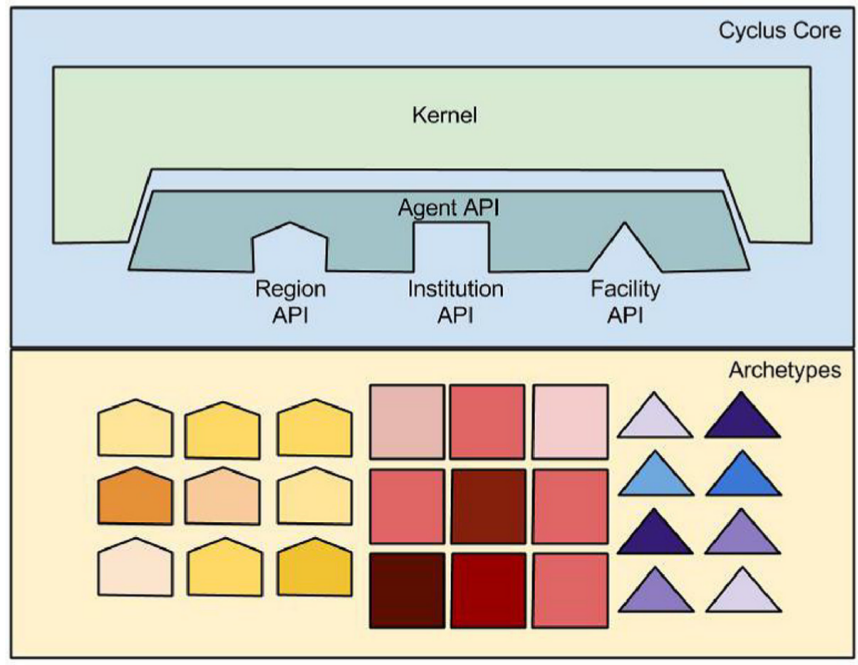
\includegraphics[width=0.7\linewidth]{images/cyclus-core}
	\caption{Visualization of the \Cyclus API for modular facilities, regions, and institutions \cite{huff_fundamental_2016}.}
	\label{fig:cyc-api}
\end{figure}

The structure seen in Figure \ref{fig:cyc-api} is largely responsible for the potential breadth of agent types of varying fidelity. Provided new agents have the appropriate material trade offers and requests,
facilities can be designed to any required fidelity.

\subsection{Archetypes}

Agents contain a hierarchy of \emph{regions, institutions, and facilities} such that \emph{regions} hold one or more \emph{institutions}. Similarly, \emph{institutions}
control \emph{facilities} necessary for the actual fuel cycle. For this work, we are most interested in the implementation of \emph{facilities} - particularly how they are defined.
Nuclear fuel cycles contain multiple variations of the same facility requiring a diverse collection of pre-designed facility process models, known as \emph{archetypes}.
These archetypes are used to define the physics and behavior of specific facility types such as reactors, reprocessing, enrichment, etc. Archetypes with pre-defined parameters are referred
to as prototypes (an AP1000 for example is a prototype). Furthermore, facilities are prototypes that have been given specific data such as deployment time, location, lifetime, etc.

\section{Pyre}

As per the goal of this project, Pyre was designed such that multiple potential pyroprocessing facilities can be modeled at medium fidelity. To accomplish this, and improve upon
the lower fidelity of the separations archetype found in \Cycamore, we inform our separation efficiencies with higher fidelity models including SSPM and AMPYRE \cite{cipiti_modeling_2012,maggos_update_2015}. The below Figure \ref{fig:flowchart} incorporates material balances for each sub-process and highlights some key parameters we
either use in the input file or look at for diversion.

\subsection{Structure of Pyre}

The archetype separates each sub-process to be handled independently, letting the user determine which aspects are necessary for their facility. We took this approach to also
allow for better handling of various waste streams. Ceramic waste must go through the electroreductor, whereas metallic fuel can go straight into the electrorefiner \cite{michael_f._simpson_developments_2012}. 
\paragraph{Governing Pyre Class} \mbox{}\\
The archetype separates each sub-process to be handled independently, letting the user determine which aspects are necessary for their facility. Each sub-process is capable
of handling its own diversion and material tracking. The streams produced from these processes are sent further through the facility, and the wastes are recorded. Waste streams are
used to verify nominal operation before being traded to a storage facility. Product streams are further refined by each sub-process until the fuel fabrication stage.
The pure uranium stream and U/TRU stream are then offered up for trade with a fuel fabricator.

\FloatBarrier

\begin{figure}[h]
	\centering
	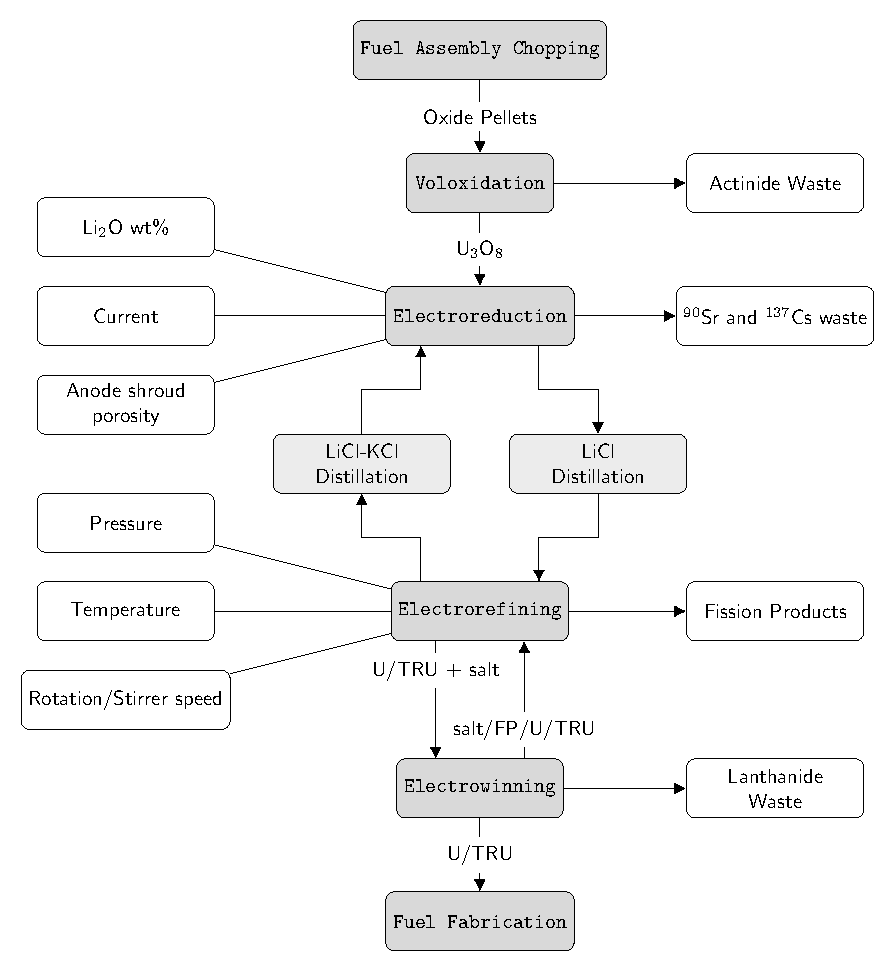
\includegraphics[width=0.9\linewidth]{images/flowchart}
	\caption{Pyre material flowchart \cite{borrelli_approaches_2017}.}
	\label{fig:flowchart}
\end{figure}

\FloatBarrier

\section{Signatures and Observables}

Before constructing a pyroprocessing archetype, appropriate signatures and observables must be determined to set as our input parameters. To identify signatures and observables 
found in a variety of pyroprocessing plants, we expand upon what was discussed in chapter 1 by looking at experimental data from electrochemical plants. The primary resources are from 
INL, KAERI, and ANL \cite{lee_korean_2011,flowsheet_1998,michael_f._simpson_developments_2012,li_electrorefining_2005}. We break up these parameters into two distinct categories: direct and indirect, corresponding to signatures and observables, respectively. If the inspector has direct access to material these are referred to as signatures, whereas, indirect monitoring, such as
power draw or thermal imaging, represent a lower level of access. 

Potentially trackable signatures and observables include truck deliveries and  power draw  \cite{Hou_2016,Yilmaz_2016}. This list is expanded upon in Table \ref{tab:params} to include pyroprocessing parameters. For this work we narrow down the list to more facility specific parameters rather than observables like the parking lot or truck movement. We also use this table
to determine the most common operational settings such as temperature, pressure, current and flow rate.

\begin{table}[h]
	\centering
	\begin{tabularx}{0.9\linewidth}{llcr}
		\hline
		\textbf{Sub-process} & \textbf{Parameters} & \textbf{S \& O} & \textbf{Refs} \\
		\hline
		Voloxidation & Volume & Tritium & \cite{jubin_spent_2009} \\
		& Oxidant & $^{14}$C & \cite{flowsheet_1998} \\
		& Flow Rate &  $^{129}$I &  \\
		& Temperature & $^{85}$Kr &  \\
		& Time & Actinides & \\ \hline
		Electroreduction & Volume & $^{90}$Sr & \cite{borrelli_approaches_2017} \\
		& Batch Size & $^{135}$Cs & \cite{flowsheet_1998} \\
		& Li$_2$O wt\% & $^{137}$Cs & \cite{choi_electrochemical_2015} \\
		& Current & Power Draw & \cite{lee_korean_2011} \\
		& Porosity & Shipments & \cite{lee_modeling_2016} \\
		& Distillation Speed & Throughput & \\ 
		& Time & & \\ \hline
		Electrorefining & Volume & Fission Products & \cite{lee_advanced_2008} \\
		& Time & Power Draw & \cite{lee_korean_2011} \\
		& Material & Waste Salt & \cite{flowsheet_1998} \\
		& Anode Rotation & Vacuum Pressure & \cite{koyama_development_2012} \\
		& Stirrer Speed & Temperature & \cite{kim_development_2013} \\
		& Pressure & Throughput & \\
		& Temperature & & \\ \hline
		Electrowinning & Current & Power Draw & \cite{flowsheet_1998} \\
		& Shroud Material & Cadmium Waste & \cite{lee_korean_2011} \\
		& Time & Fission Products & \cite{borrelli_approaches_2017} \\
		& Flow Rate & Lanthanides & \\
		&  & $^{135}$Cs & \\
		&  & $^{137}$Cs & \\ \hline
		Facility & Throughput & Shipments & \\
		& Batch Size & Parking Lot & \\
		& & Thermal Image & \\
		\hline
	\end{tabularx}
	\caption {Archetype inputs and signatures \& observables at each sub-process.}
	\label {tab:params}
\end{table}

\subsection{Material Balance}
We take a material balance area over each sub-processes using the signatures and observables identified in Table \ref{tab:params}. 
These balance areas are shown through flowcharts describing operational parameters in green, and signatures and observables in red. 

\paragraph{Voloxidation} \mbox{}\\
\gls{LWR} fuel must be treated and separated before proceeding with electrolytic processes. Uranium dioxide heated to 
500$^{\circ}$C is converted to $U_3O_8$ while noble gases, carbon, and tritium are collected to decay in storage. 
Actinides are also converted to their stable oxide forms and a majority are removed \cite{flowsheet_1998,jubin_spent_2009}. 
Heating uranium dioxide above 800$^{\circ}$C increases voloxidation throughput.
Cycling oxidants between H$_2$ and air also improves the U$_3$O$_8$ reaction rate \cite{jubin_spent_2009}.

\begin{figure}[h]
	\centering
	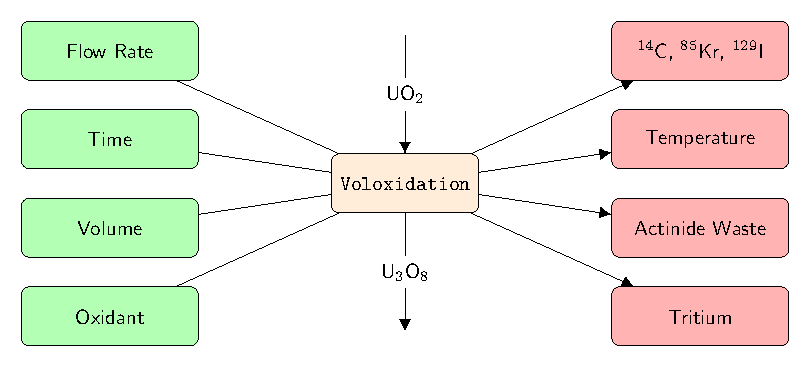
\includegraphics[width=0.9\linewidth]{images/volox}
	\caption{Voloxidation material balance area \cite{jubin_spent_2009}.}
	\label{fig:volox}
\end{figure}

\paragraph{Electroreduction} \mbox{}\\
The oxidant is converted into metallic fuel through electroreduction to be further refined through electrorefining and electrowinning. 
Yellowcake, created in voloxidation, enters the cathode, a negatively charged metal basket. 
A current density between 100 and 500 mA/cm$^2$ is applied to the anode in a molten LiCl salt. 
The electrolytic reduction process primarily results in diffusion of Cs, Ba and Sr, along with reduction and conversion of Zr into metallic form \cite{choi_electrochemical_2015,flowsheet_1998}.
Electroreduction can further improve its throughput by adding Li$_2$O as a catalyst; this catalyst also prevents dissolution 
of the anode \cite{choi_electrochemical_2015}. Since Li$_2$O is used to speed up the reaction,
the operators could add more oxide than reported to \gls{IAEA}. More frequent shipments 
of lithium oxide can be tracked as an observable to match records.

\begin{figure}[h]
	\centering
	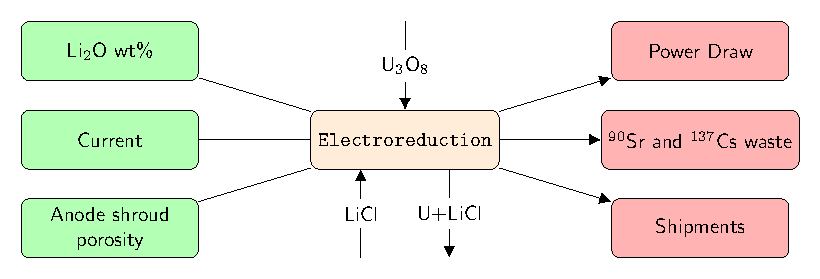
\includegraphics[width=0.9\linewidth]{images/reduction}
	\caption{Reduction material balance area \cite{lee_advanced_2008}.}
	\label{fig:reduction}
\end{figure}

\paragraph{Electrorefiner} \mbox{}\\
Once in metallic form, electrorefining electrochemically separates uranium and TRUs for fuel fabrication.
The uranium and salt mixture from reduction is fed into an anode basket suspended in a graphite cathode. 
A LiCl-KCl eutectic is used as an electrolyte above 500$^{\circ}$C \cite{flowsheet_1998,lee_korean_2011}. 
Uranium dissolves at the anode to recombine at the cathode as metallic uranium.
Waste TRUs and lanthanides are in a soluble chloride form  while fission products and cladding remain in the anode
basket. Finally, actinides and fission products are removed from the cladding electrochemically \cite{lee_korean_2011}.

Lee et al. \cite{lee_advanced_2008} show decreasing system pressure improves removal efficiency. 
Temperature, however, exhibits the opposite effect: as temperature decreases so does salt removal. This comes into effect 
particularly depending on instrumentation and containment material choice \cite{lee_advanced_2008}. 
Iron, for example, limits operating temperature because a eutectic forms at 725$^{\circ}$C \cite{chapman_revision_1984}.
In facilities where iron equipment is present, temperatures are limited to 700$^{\circ}$C, hindering efficiency. 
Cathode arrangement and anode rotation speed also affect the collection of uranium 
dendrites \cite{lee_advanced_2008}. A central stirrer mixes uranium dendrites stuck on 
the vessel, improving separation efficiency and increasing throughput. 

\begin{figure}[h]
	\centering
	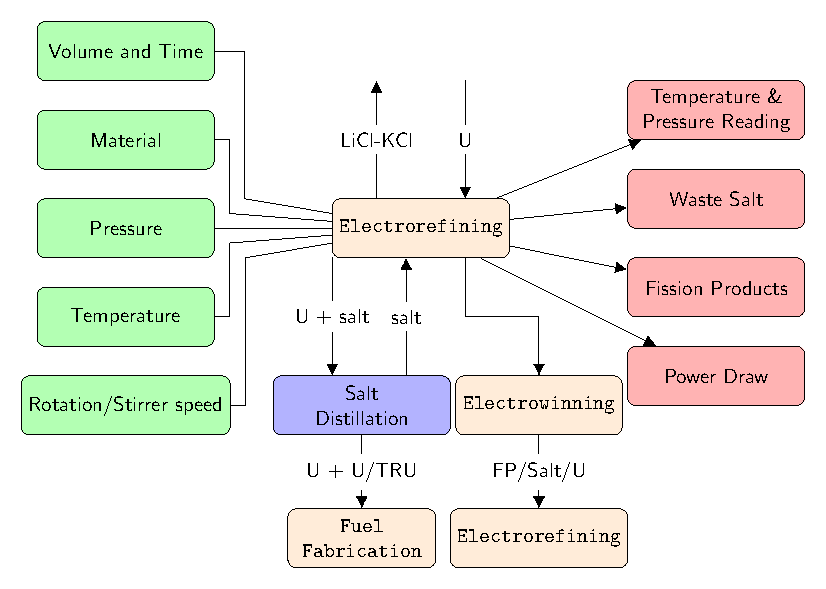
\includegraphics[width=0.85\linewidth]{images/refining}
	\caption{Refining material balance area \cite{lee_advanced_2008}.}
	\label{fig:refining}
\end{figure}

The electrorefining process also produces a fission product waste stream which requires monitoring. 
The following products are produced and tracked in \gls{PyRe} at this step: Tc, Ag, Pd, Rh, Ru, Mo, and Zr \cite{flowsheet_1998}. 
Uranium and \gls{TRU} product streams separated at this stage are sent to fuel fabrication, while the remaining salt is reformed as an oxidant and recirculated.
Separation efficiencies are taken after recirculation and treated as a once-through cycle. 

\paragraph{Electrowinner} \mbox{}\\
Molten salt containing \glspl{TRU} from electrorefining is separated through electrowinning. This process separates trace uranium quantities, lanthanides and fission products. 
At 500$^{\circ}$C there is approximately 99 wt\% reduction in actinides and lanthanides \cite{flowsheet_1998}. 
Throughput also depends on material choice for the inert electrodes, impacting separation 
efficiency \cite{koyama_development_2012}. A shroud surrounds the anode to provide a path for O$^{2-}$ ions to the anode and 
prevent Cl$_2$ from corroding the anode \cite{kim_development_2013,choi_electrochemical_2015}. Optimum operating current 
depends on material choice for the anode shroud since a nonporous shroud limits ion pathways to the anode contact points.
Higher porosity corresponds to free ion paths and a higher current. Increased currents reduce the separation time for electroreduction and electrowinning \cite{choi_electrochemical_2015}.

\begin{figure}[h] 
	\centering
	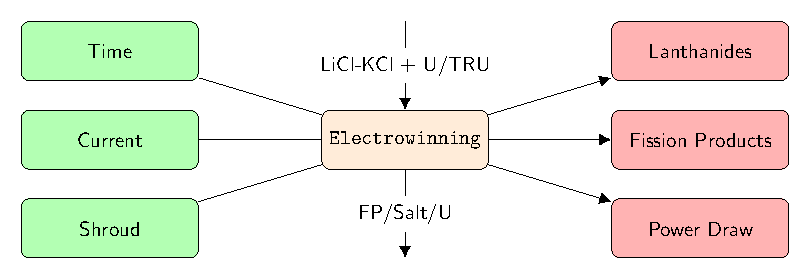
\includegraphics[width=0.8\linewidth]{images/winning}
	\caption{Winning material balance area.}
	\label{fig:winning}
\end{figure}

\subsection{Waste Forms}

Waste from pyroprocessing exists in three main waste streams in which IAEA can directly measure their \emph{signatures}. Monitoring signatures require direct access to the waste streams.
These techniques vary depending on the waste form. Leading approaches include non-destructive assay, multiplicity counting, and a plutonium to curium ratio measurement \cite{lee_determination_2012,noauthor_non-destructive_nodate}.

\paragraph{Diverter} \mbox{}\\
Figure \ref{fig:diverttype} shows the difference between nefarious diversion, in gray, and operator diversion, in orange. The gray line shows normal operation where diversion occurs
through the shipment, and can be detected by a discrepancy in shipment records. The more difficult case to handle, shown in orange, imagines an inside man altering operational settings
to increase product over reported quantities. The scenario we are concerned with is operator diversion; we wish to determine the most important points in the plant to monitor for potential
diversion. A side effect of this goal is that we must be able to detect diversion by changing key operational settings.

\FloatBarrier

\begin{figure}[h]
	\centering
	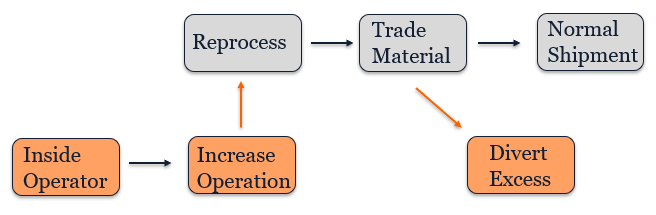
\includegraphics[width=0.8\linewidth]{images/westphal-diversion}
	\caption{A flowchart demonstrating the main forms of material diversion.}
	\label{fig:diverttype}
\end{figure}

\Cyclus does not natively handle diversion from inside facilities as required for the goals for Pyre. We implemented a higher fidelity diversion model through the
diverter class to handle operator and nefarious diversion. This class is specific to the Pyre archetype currently, as the diversion facility must be set up to allow it.
The diverter class' goal is to inform the Pyre facility what parameters are being changed to divert material. The algorithm used for this can be seen in Figure \ref{fig:divflow}
which inputs the sub-process that contains an inside man, the parameters he has access to, and how much material he wishes to divert. The diverter directs this information to the
appropriate sub-process which then uses a bisection function to determine the parameter value associated with the new product.

\FloatBarrier

\begin{figure}[h]
	\centering
	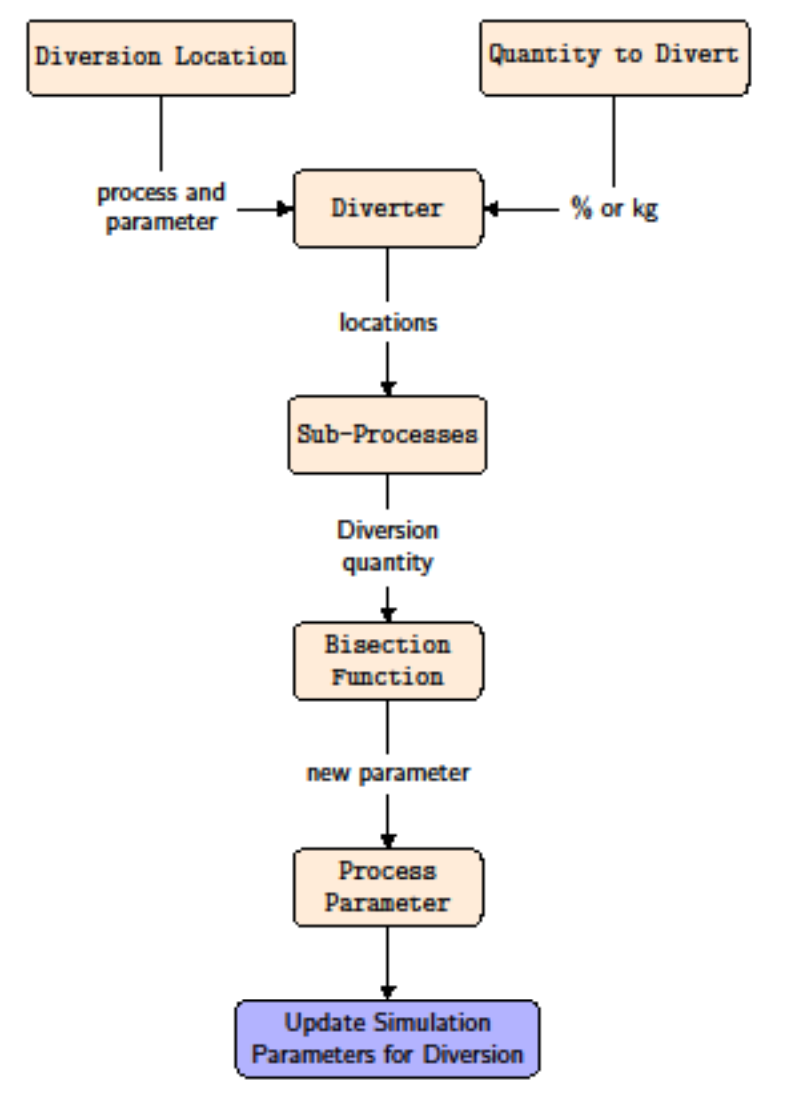
\includegraphics[width=0.65\linewidth]{images/divertflow}
	\caption{Pyre diverter class flowchart.}
	\label{fig:divflow}
\end{figure}

\subsection{User Input}
Pyre, as with all \Cyclus archetypes, is fully configurable through the text-based input file. The input consists of the operational settings shown in Table \ref{tab:params}
and the separation efficiency for each isotope. The efficiency input for each sub-process corresponds to that facility's ideal state. Operational settings act as a capacity factor,
reducing the overall efficiency to match those seen in test facilities. This input structure allows users to follow predefined example facilities, or input their own separation
efficiencies. As a result of this work, input files for PRIDE, INL, and ANL based facilities have been generated. However, a user can also input their own parameter relationship equations
if those provided do not accurately reflect their facility model.
%\chapter[Simulating Fuel Cycles]{Simulating Fuel Cycles}
\section{Simple Verification}

\begin{figure}
	\centering
	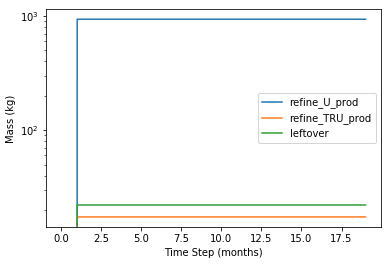
\includegraphics[width=\linewidth]{images/timeseries-prod}
	\caption{Product time series of a simple simulation.}
	\label{fig:timeseries-prod}
\end{figure}

\begin{figure}
	\centering
	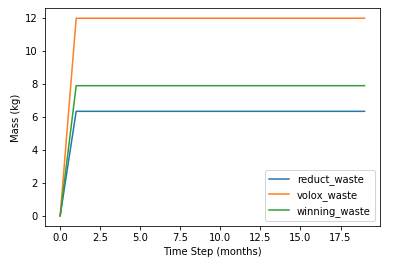
\includegraphics[width=\linewidth]{images/timeseries-waste}
	\caption{Waste time series of a simple simulation.}
	\label{fig:timeseries-waste}
\end{figure}

\begin{figure}
	\centering
	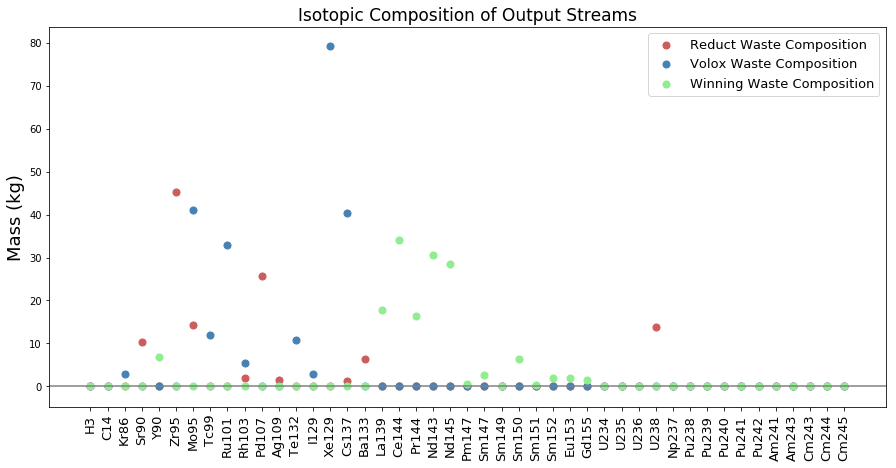
\includegraphics[width=\linewidth]{images/avg-isotope-comp}
	\caption{Isotopic Composition of Average Waste Streams}
	\label{fig:avg-isotope-comp}
\end{figure}

\begin{figure}
	\centering
	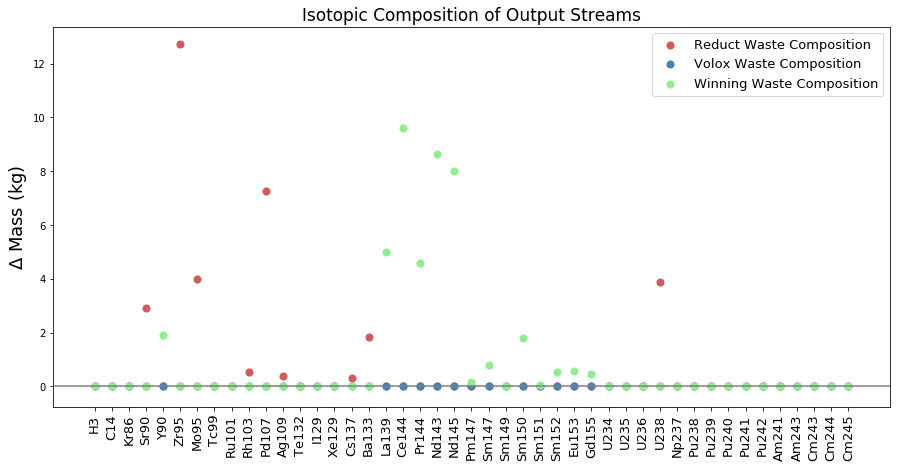
\includegraphics[width=\linewidth]{images/current-isotope-comp}
	\caption{Isotopic Composition of Current Diverted Waste Streams}
	\label{fig:current-isotope-comp}
\end{figure}

\begin{figure}
	\centering
	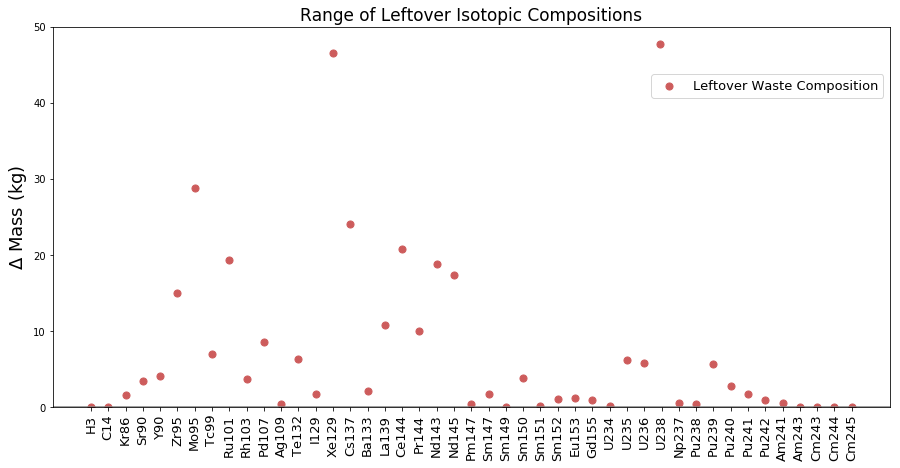
\includegraphics[width=\linewidth]{images/isotopic-comp-range}
	\caption{Range of Isotopic Values}
	\label{fig:isotopic-range}
\end{figure}

\section{US Fuel Cycle}
%\chapter[Diversion Detection]{Diversion Detection}

The second aspect of this work identifies locations sensitive to diversion in a generic pyroprocessing facility. This work leverages two approaches: applying
a cumulative sum detection algorithm and performing sensitivity analysis on key facility parameters. 
\section{Cumulative Sum}

\subsection{Requirements of Diversion Detection}


The cumulative sum method (CUSUM) applied to Pyre was chosen to fit the following requirements: function with minimal prior information, have online diversion detection
capabilities, and fit a modular approach. The CUSUM change detection algorithm calculates expected mean value of an observed data stream as shown by the following equations \cite{basseville_detection_1993}.

\begin{align}
	f_{t+1} &= max(0, f_t + x_t - \mu - \delta) \\
	\intertext{Where}
	x_t &= \mbox{observed data at time t} \nonumber \\
	\mu &= \mbox{approximated mean of x} \nonumber \\
	\delta &= \mbox{acceptable change} \nonumber
\end{align}

This general function adds new observed values to the calculated mean. If the value is within a region of allowable change, typically 3$\sigma$, the change is not reported. 
We favor this online diversion detection capability in an effort to achieve timely detection goals set by the IAEA \cite{international_atomic_energy_agency_implications_2004}.
These intermittent inspections only have access to portions of the complete data stream, thus we aim to mimic reality as closely as possible. In addition, we need this
algorithm to work on a variety of facilities with various active sub-processes.

\subsection{Limitations of selected method}

The CUSUM approach is not without its drawbacks: since there is no prior data assumed we must generate a reasonable mean from observed data before being able to detect diversion. In this work
we assume a startup time of approximately 6 months before an appropriate mean can be developed. The next limitation faced with this approach is that CUSUM assumes one can only observe one data stream at a time, while
real inspections take a wide range of conditions into account. This concern is addressed by using sensitivity analysis, as seen later in this chapter, to inform on the most crucial
sub-processes or settings. 

CUSUM relies on a variable mean and noise to obscure possible change points. When a simulator knows the exact value at each time step, without human reporting or measurement error, change 
detection becomes trivial. To best represent the uncertainty inherent in material accountancy measurement, noise is artificially created when the CUSUM class reads data. This way \Cyclus retains its constant operating value while the change point
has potential to be obscured by measurement error. These detector uncertainties are assumed from common non-destructive and destructive assay practices used by the SEE LANL safeguards training course \cite{root_see_2019}.

\section{Verification}

To test operator diversion capabilities, we ran the EG01-EG24 transition scenario shown in chapter 3 with inside operators. The scenario described in Table \ref{tab:setup} contains an LWR and SFR configuration for Pyre. Each prototype siphoned material with different quantities and frequencies to demonstrate its reconfigurability. The pyroprocessing facility that exclusively accepts LWR fuel siphoned off 5\% every 10 timesteps while the facility that only accepts SFR fuel siphoned off 1\% excess every other timestep.  Results for this scenario are shown in Figure \ref{fig:divertmat}.

\begin{figure}
	\centering
	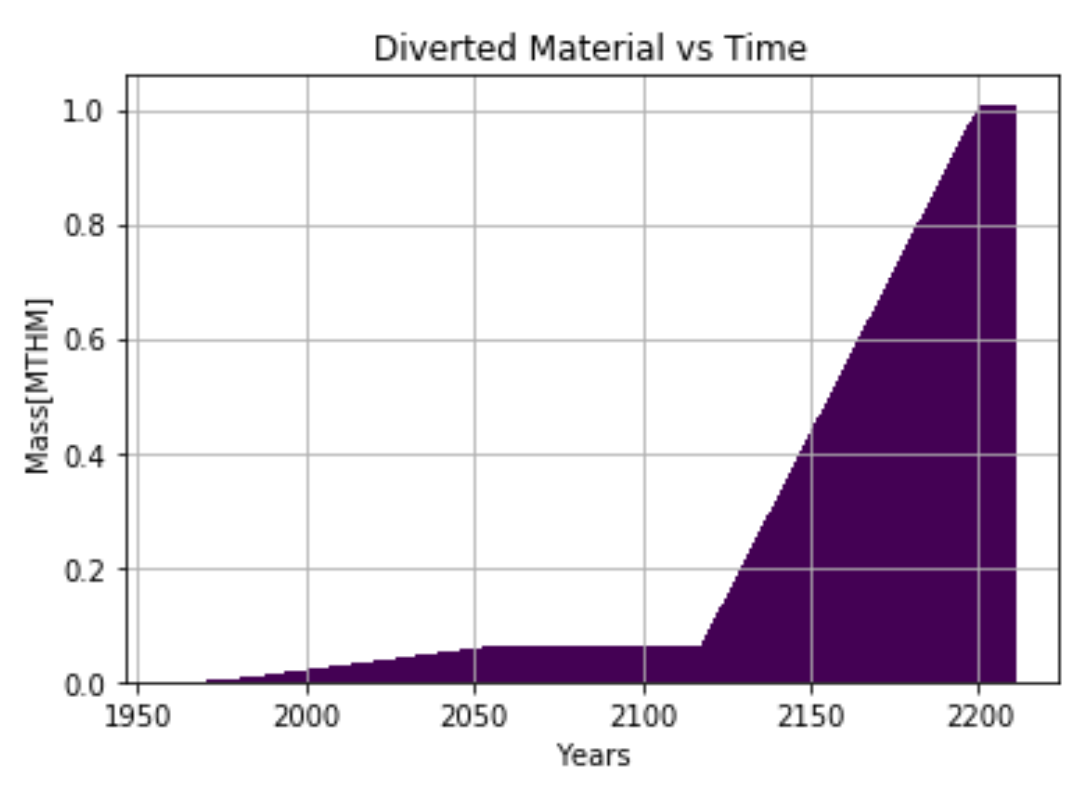
\includegraphics[width=0.9\linewidth]{images/divertmat}
	\caption{A timeseries of diverted material from transition scenario EG01-EG24.}
	\label{fig:divertmat}
\end{figure}

\section{Sensitivity Analysis}

The sensitivity analysis approach in this work illuminates the limits of monitoring future pyroprocessing facilities. This work relies on Dakota to alter \Cyclus input files and provides a number of statistics packages, allowing us to easily
run batches of scenarios. To properly use Dakota with \Cyclus, we must use DCWrapper, which uses python to interface between Dakota and \Cyclus' xml input files. 
Key parameters were sampled over a range of values for diversion to verify the archetype's capabilities and identify operational ranges. The range for each parameter is shown in Table \ref{tab:range}. 

\begin{table}[h]
	\centering
	\begin{tabularx}{0.85\linewidth}{lccc}
		\hline
		\textbf{Parameter} & \textbf{Lower Bound} & \textbf{Upper Bound} & \textbf{Units} \\
		\hline \hline
		Electrorefiner Temp & 750 & 1000 & $^\circ C$ \\ \hline
		Electrorefiner Pressure & 100 & 760 & mTorr \\ \hline
		Electrorefiner Stirrer Speed & 0 & 100 & rpm \\ \hline
		Electrowinner Current & 5 & 10 & Amps \\ \hline
		Electrowinner Flow Rate & 2 & 4.5 & cm/s \\ \hline
		Electrowinner Process Time & 1 & 4 & hours \\ \hline
	\end{tabularx}
	\caption {Range of Each Sensitivity Analysis Parameter Sample.}
	\label {tab:range}
\end{table}

Parameters were selected from the most attractive
sub-processes for diversion, the electrorefiner and electrowinner. These two processes are responsible for the production of Uranium and U/TRU ingots, therefore sensitivity analysis was run
on each of their key parameters: Temperature, Current, Flowrate, Pressure, Stirrer Speed, and Reprocessing Time. Six samples were selected at regular intervals across the range of each parameter. For each setting we observe how much material can be diverted within a month.

\subsection{Electrorefiner Temperature}

The first setting for consideration is the electrorefiner's temperature. As discussed in methodology, the range for this setting is 500 to 1000 $^\circ C$ with typical operation above 750 $^\circ C$. These values can be seen isotopically in Figure \ref{fig:ref-temp-sa}.
The 750 $^\circ C$ stream is then subtracted from the sampled streams to determine the impact of increasing temperature on divertable material.
While temperature is a key aspect to the electrorefiner, Figure \ref{fig:ref-temp-diff} shows that temperatures approaching 1000 $^\circ C$ result in diminishing returns.

\begin{figure}
	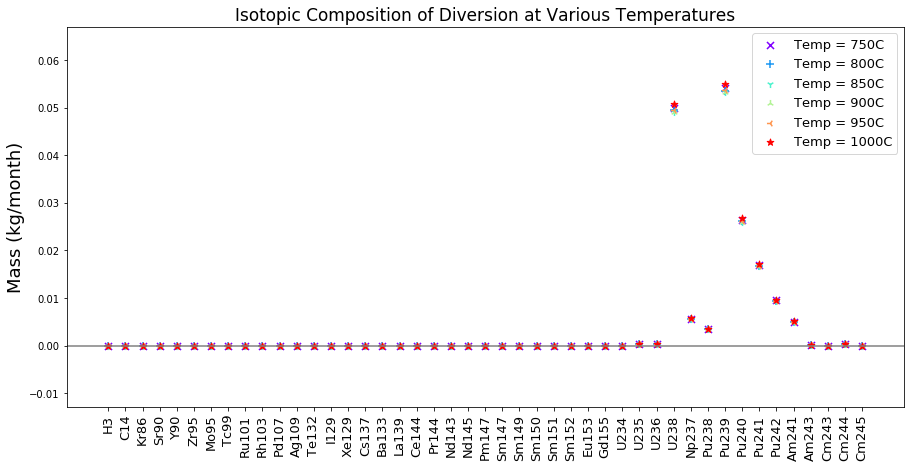
\includegraphics[width=\linewidth]{images/temperature-sa-comp}
	\caption{Isotopic composition of the diverted material stream at various electrorefiner temperatures.}
	\label{fig:ref-temp-sa}
\end{figure}

\begin{figure}
	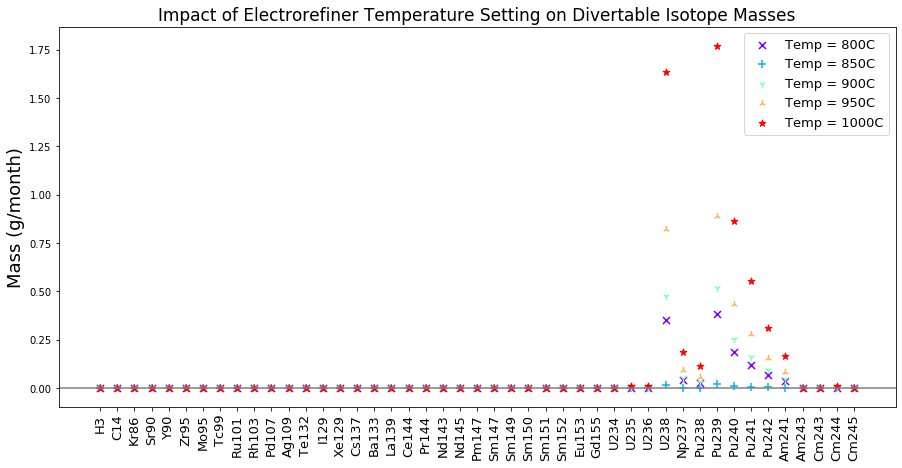
\includegraphics[width=\linewidth]{images/temperature-sa-diff}
	\caption{Isotopic composition of the diverted material stream at various electrorefiner temperatures.}
	\label{fig:ref-temp-diff}
\end{figure}

\subsection{Electrorefiner Pressure}

Available in advanced electrorefiners, lower vacuum pressure can improve separation efficiency as well. Similar to our analysis of temperature, isotopic compositions of
divertable material can be seen in Figure \ref{fig:ref-press-sa}. Our baseline for the comparison is atmospheric pressure as this will represent facilities lacking this
functionality. 

\begin{figure}
	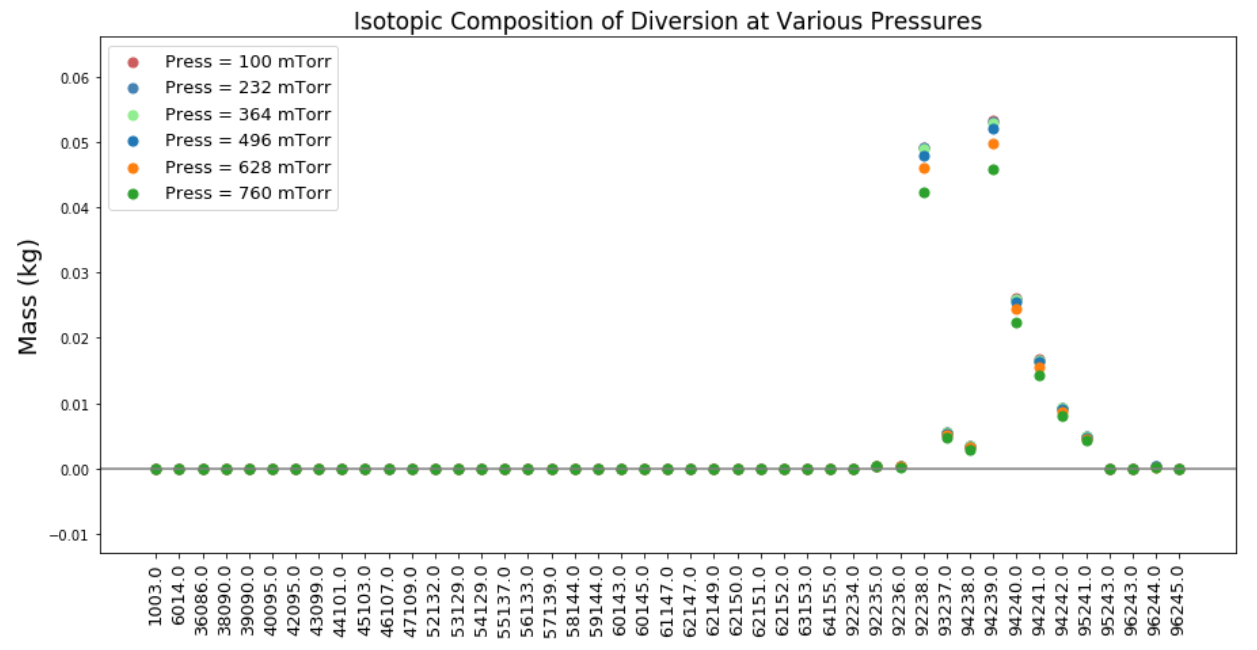
\includegraphics[width=\linewidth]{images/pressure-sa-comp}
	\caption{Isotopic composition of the Diverted material stream at various electrorefiner pressures.}
	\label{fig:ref-press-sa}
\end{figure}

\begin{figure}
	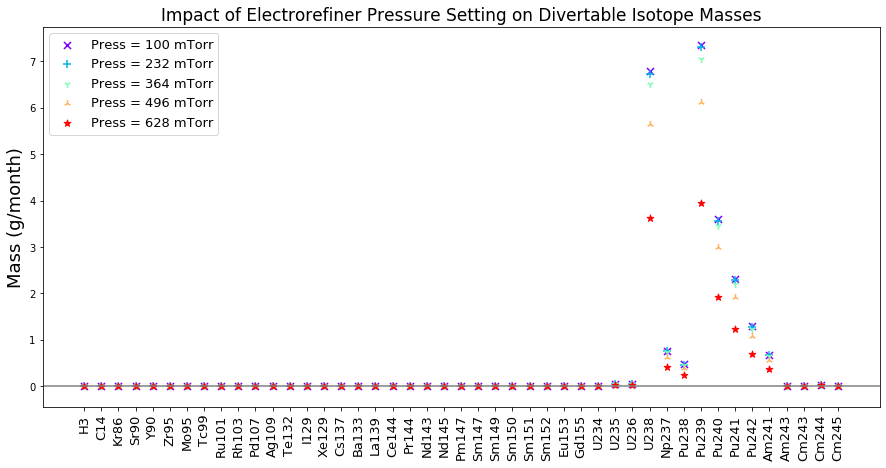
\includegraphics[width=\linewidth]{images/pressure-sa-diff}
	\caption{Isotopic composition of the Diverted material stream at various electrorefiner pressures.}
	\label{fig:ref-press-diff}
\end{figure}

\subsection{Electrorefiner Stirrer Speed}

The central stirrer is another setting particular to advanced refining techniques \cite{lee_advanced_2008}. Pyre tracks this parameter since adding a stirrer to processes can be a simple procedure. Figure \ref{fig:ref-rot-sa} shows the isotopic distribution associated with a
range of different stirrer speeds. Stirrer speed higher than 100 rpm results in uranium dendrites returning
to the salt. Therefore, in Figure \ref{fig:ref-rot-diff} this work took 0 rpm as our baseline to represent facilities with no stirrer, and 100 rpm as our maximum. 

\begin{figure}
	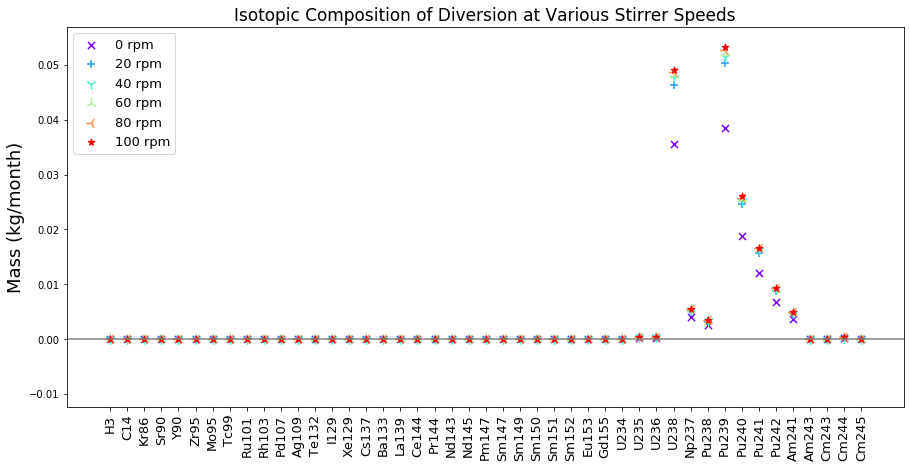
\includegraphics[width=\linewidth]{images/rotation-sa-comp}
	\caption{Isotopic composition of the diverted material stream at various central stirrer speeds.}
	\label{fig:ref-rot-sa}
\end{figure}

\begin{figure}
	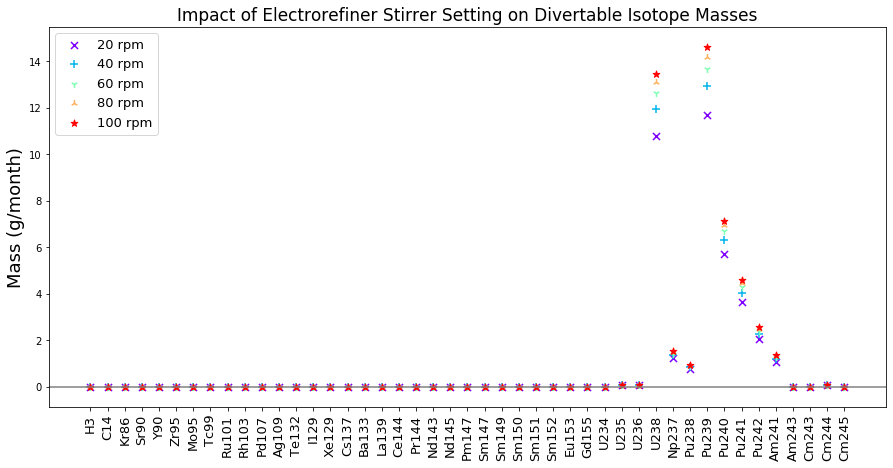
\includegraphics[width=\linewidth]{images/rotation-sa-diff}
	\caption{Isotopic composition of the diverted material stream at various central stirrer speeds.}
	\label{fig:ref-rot-diff}
\end{figure}

\subsection{Electrowinner Current}

The primary setting for the electrowinning sub-process is the current. The current's relationship with efficiency decreases in separation beginning around 10 A.
This is seen in Figures \ref{fig:win-cur-sa} and \ref{fig:win-cur-diff} as 10 A is below the efficiency of 5 A. This relationship occurs due to increasing voltage no longer aiding in separation of some lanthanides as described in chapter 2. Figure \ref{fig:win-cur-diff} shows that the key operating range lies within 6-8 A.

\begin{figure}
	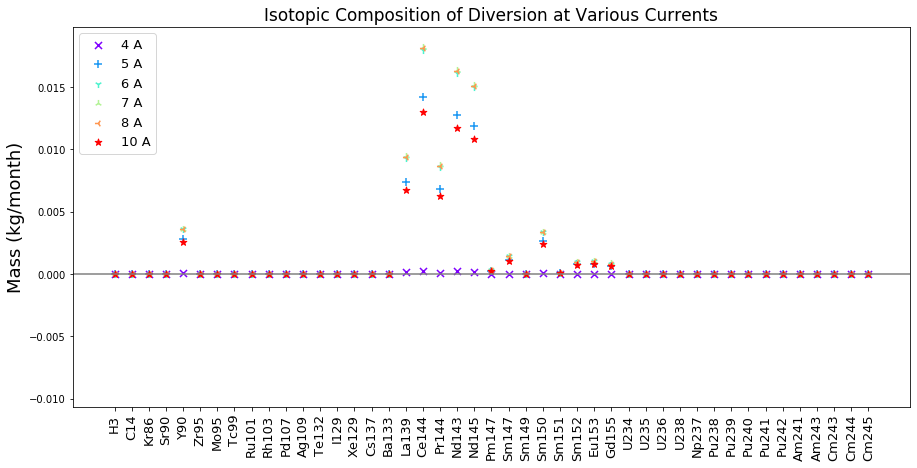
\includegraphics[width=\linewidth]{images/current-sa-comp}
	\caption{Isotopic composition of the diverted material stream at various electrowinner currents.}
	\label{fig:win-cur-sa}
\end{figure}

\begin{figure}
	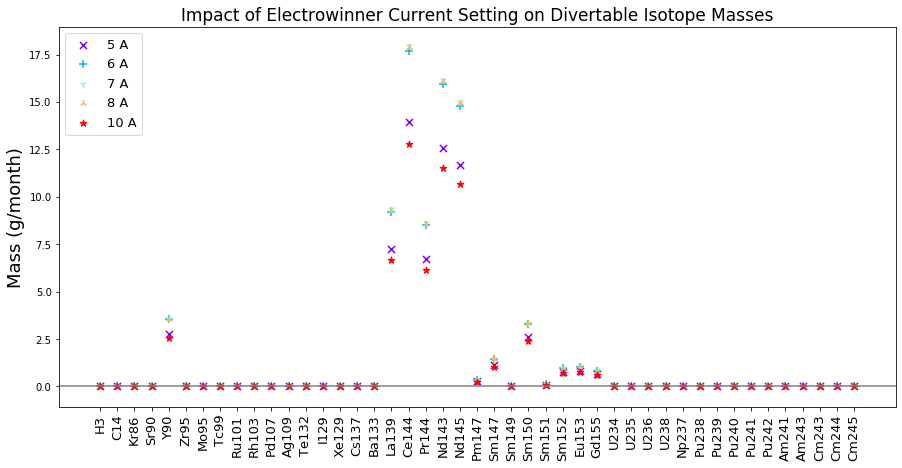
\includegraphics[width=\linewidth]{images/current-sa-diff}
	\caption{Isotopic composition of the diverted material stream at various electrowinner currents.}
	\label{fig:win-cur-diff}
\end{figure}

\subsection{Electrowinner Flow rate}

Similar to the central stirrer of the electrorefiner, increasing the flow rate through the electrowinner can aid removal of additional lanthanides and TRU. Flow rates shown are linear rates, with the bounds corresponding to minimum and maximum values tested in experimental facilities. Figures \ref{fig:win-flow-sa} and \ref{fig:win-flow-diff} demonstrate a steady increase in removal rates with increasing flow.

\begin{figure}
	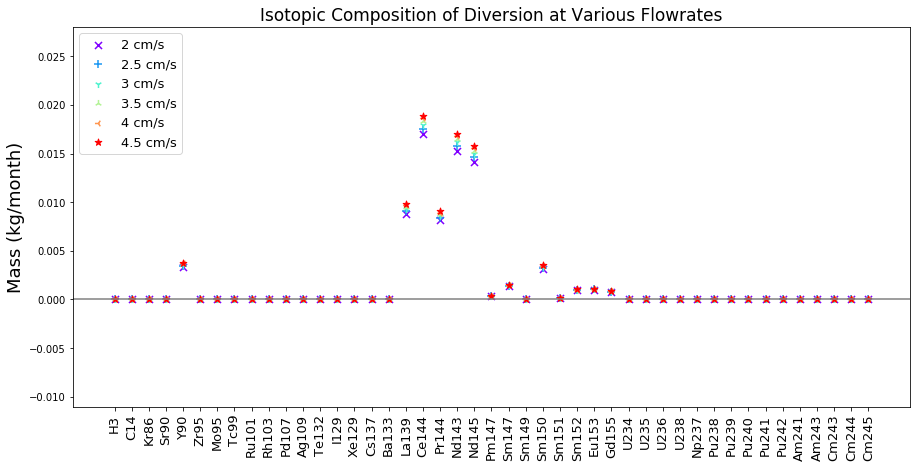
\includegraphics[width=\linewidth]{images/flowrate-sa-comp}
	\caption{Isotopic composition of the diverted material stream at various electrowinner flowrates.}
	\label{fig:win-flow-sa}
\end{figure}

\begin{figure}
	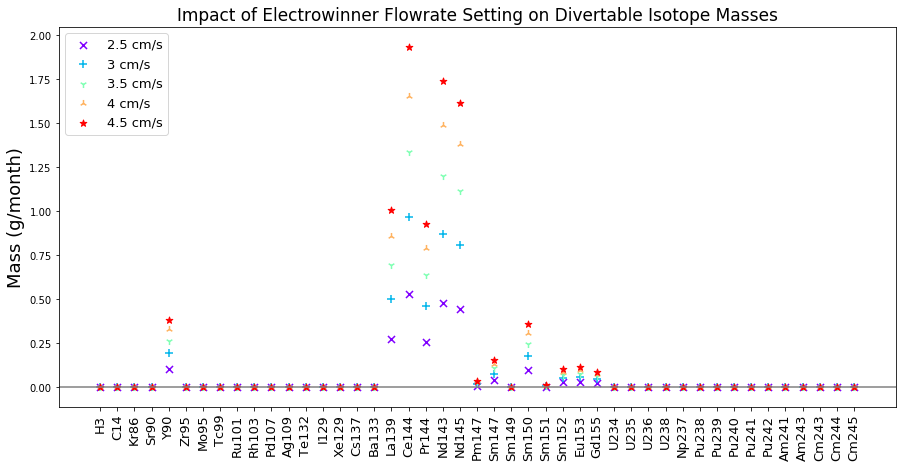
\includegraphics[width=\linewidth]{images/flowrate-sa-diff}
	\caption{Isotopic composition of the diverted material stream at various electrowinner flowrates.}
	\label{fig:win-flow-diff}
\end{figure}

\subsection{Electrowinner Reprocessing Time}

The final setting we chose to observe was time spent in the electrowinner. We chose this sub-process since it is closely related to the U/TRU product stream. Comparing Figure \ref{fig:win-time-diff} to Figure \ref{fig:win-flow-diff}, we can see that increasing 
reprocessing time results in more divertable material. 

\begin{figure}
	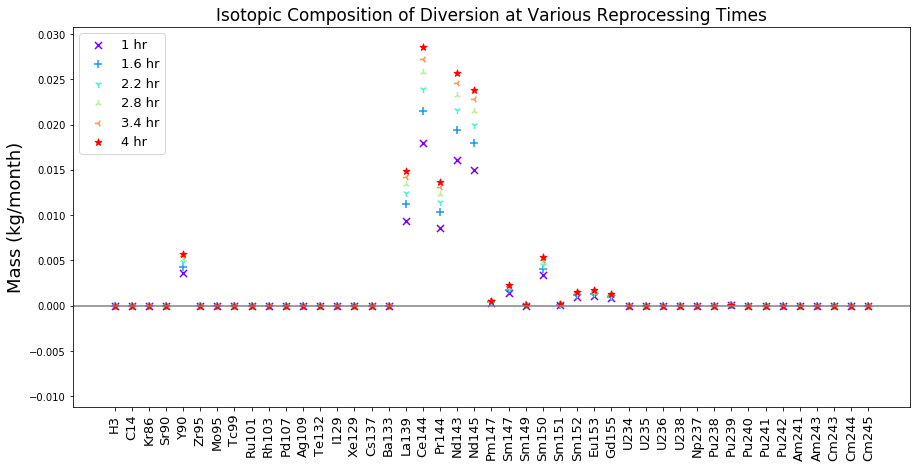
\includegraphics[width=\linewidth]{images/time-sa-comp}
	\caption{Isotopic composition of the diverted material stream at various electrowinner reprocessing durations.}
	\label{fig:win-time-sa}
\end{figure}

\begin{figure}
	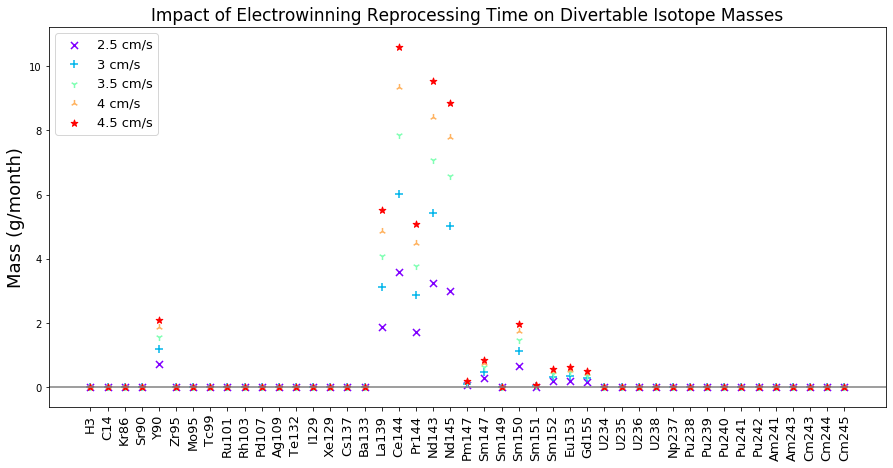
\includegraphics[width=\linewidth]{images/time-sa-diff}
	\caption{Isotopic composition of the diverted material stream at various electrowinner reprocessing durations.}
	\label{fig:win-time-diff}
\end{figure}

\section{Parameter Comparison}

The material increase due to the previous six operational settings was normalized against their respective baseline
to determine the most impactful process parameters. Table \ref{tab:compare} summarizes these values.

\begin{table}[h]
	\centering
	\begin{tabularx}{0.9\linewidth}{lcccccc}
		\hline
		\textbf{Sample} & \textbf{ER} & \textbf{ER} & \textbf{ER} & \textbf{EW}
		& \textbf{EW} & \textbf{EW} \\
		& \textbf{Temp} & \textbf{Pressure} & \textbf{Stir Speed} & \textbf{Current} & \textbf{Flow rate} & \textbf{Time} \\
		\hline \hline
		1 & 0.036 & 8.589 & 30.284 & 5.684 & 3.136 & 20.030 \\ \hline
		2 & 0.715 & 13.336 & 33.542 & 7.216 & 5.699 & 33.602 \\ \hline
		3 & 0.975 & 15.393 & 35.447 & 7.308 & 7.866 & 43.879 \\ \hline
		4 & 1.672 & 15.912 & 36.799 & 7.281 & 9.743 & 52.154 \\ \hline
		5 & 3.328 & 16.047 & 37.848 & 5.202 & 11.398 & 59.080 \\ \hline
	\end{tabularx}
	\caption {Comparison of operational settings' impact on divertable material (shown in
		\% difference compared to baseline values). Where ER and EW represent electrorefiner and electrowinner respectively.}
	\label {tab:compare}
\end{table}

Sensitivity analysis for each setting is split into corresponding samples to reflect increasing efficiency. As we observed earlier, temperature and current, although primary settings, 
do not result in significant increase in separated material. Temperature alterations result in diminishing returns, as a drastic increase of heat is required for noticeably improved efficiency. Notably,
the most impactful electrorefiner setting is the central stirrer's speed. The stirrer  
has such a significant impact due to increasing the rate of separation, and improving overall
efficiency. Comparing the stirrer and pressure separation efficiency illuminates the stirrer's significance. Reducing pressure to 100 mTorr results in a 16\% increase in material while a stirrer at 20 rpm nearly doubles that at 30.284\% increase.
Separation efficiency due to changes in current plateaus because the process is limited by reaction rate. Increasing electrowinner current does not affect opportunity to react as flowrate and time can be seen to do. 
A trend noticed in these settings is those which allow more interaction between the salt and waste see a more significant increase in product. 

While the rest also result in
improved efficiency, they require a larger change in operation to meet the same increased separation.
%\chapter{Conclusion}

This thesis was motivated by a lack of medium fidelity pyroprocessing plants in current fuel cycle simulators \cite{borrelli_approaches_2017}. Combined with 
the need for safeguards by design in next generation nuclear fuel cycle facilities, a pyroprocessing facility with diversion capabilities fills a technological gap.
Pyre brings more detailed separations processes to nuclear fuel cycle simulators informed by more limited and specific electrochemical models such as SSPM and AMPYRE \cite{maggos_update_2015}.

\Cyclus provides a modular interface to expand and test the capabilities of reprocessing and material diversion. We developed Pyre in the C++ \Cyclus environment to leverage this
modular framework and test the facility in a key pyroprocessing transition-scenario. We ran a full US fuel cycle transitioning from LWRs to SFRs using only Pyre facilities to facilitate
this transition. We verified Pyre's role in this transition-scenario by observing the simulation's uranium utilization, TRU production, and successful fueling and operation of SFRs to
meet power demands.

%%%%%%%%%%%%%%%%%%%%%%%%%%%%%%%%%%%%%%%%%%%%%%%%%%%%%%%%%%%%%%%%%%%%%%%%%%%%%%%
% APPENDIX
%
%\appendix
%\include{apx}

\backmatter

%%%%%%%%%%%%%%%%%%%%%%%%%%%%%%%%%%%%%%%%%%%%%%%%%%%%%%%%%%%%%%%%%%%%%%%%%%%%%%%
% BIBLIOGRAPHY
%
%\bibliographystyle{IEEE_ECE}
\bibliographystyle{IEEE_ECE}
% Put references in BibTeX format in thesisrefs.bib.
\bibliography{thesisrefs}

\end{document}
\endinput
